\documentclass[tikz,border=5mm]{standalone}
%\documentclass[convert={density=300,size=1080x800,outext=.png}]{standalone}
%\documentclass[a4paper]{memoir}

\usepackage{pgfplots}
\pgfplotsset{compat=newest}
\usepgfplotslibrary{fillbetween}
\usetikzlibrary{calc,angles,positioning,intersections,quotes,decorations.markings,backgrounds,patterns}

\begin{document}

% ------------------------------------------------------------------------------------------------------------------------
% CARTESIAN COORDINATE SYSTEM
% ------------------------------------------------------------------------------------------------------------------------

\begin{tikzpicture} [scale=1.0]
  \begin{axis}[
    name = plot1,
%    title=Cartesian Coordinate System,
    width = 20cm, 
    height = 20cm,
    axis lines=middle,
    axis equal image,
    axis on top = true, axis x line = middle, axis y line = middle,
    xmin = -11, ymin = -11, xmax = 11, ymax = 11,
    /pgfplots/xtick = {-10,...,10},
    /pgfplots/ytick = {-10,...,10},
    tick align = outside,
    xlabel = {$x_1$}, xlabel style = {at={(ticklabel* cs:1)},anchor = north west},
    ylabel = {$x_2$}, ylabel style = {at={(ticklabel* cs:1)},anchor = east},
    %legend entries={Constraint 1,Constraint 2,Constraint 3},
    ]
    \node at (6,5) {\Huge{I}};
    \node at (6,-5) {\Huge{II}};
    \node at (-6,-5) {\Huge{III}};
    \node at (-6,5) {\Huge{IV}};
  \end{axis}
\end{tikzpicture}

% ------------------------------------------------------------------------------------------------------------------------

% ------------------------------------------------------------------------------------------------------------------------
% CARTESIAN COORDINATE SYSTEM - FIRST QUADRANT
% ------------------------------------------------------------------------------------------------------------------------

\begin{tikzpicture} [scale=1.0]
  \begin{axis}[
    name = plot1,
%    title=Cartesian Coordinate System - First Quadrant,
    width = 20cm, 
    height = 20cm,
    axis lines=middle,
    axis equal image,
    axis on top = true, axis x line = middle, axis y line = middle,
    xmin = 0, ymin = 0, xmax = 21, ymax = 21,
    /pgfplots/xtick = {0,...,20},
    /pgfplots/ytick = {0,...,20},
    tick align = outside,
    xlabel = {$x_1$}, xlabel style = {at={(ticklabel* cs:1)},anchor = north west},
    ylabel = {$x_2$}, ylabel style = {at={(ticklabel* cs:1)},anchor = east},
    ]
%	\addplot[blue,dashed, line width = 1] coordinates {(8,0)(8,6)(0,6)};
%    \filldraw[blue] (8,6) circle (2pt) node[anchor=south west] {$(x_1 = 8,x_2 = 6)$};
  \end{axis}
\end{tikzpicture}

% ------------------------------------------------------------------------------------------------------------------------

% ------------------------------------------------------------------------------------------------------------------------
% LABOR CONSTRAINT LINE
% ------------------------------------------------------------------------------------------------------------------------

\begin{tikzpicture} [scale=1.0]
  \begin{axis}[
    name = plot1,
    title=Labor Constraint Line,
    width = 20cm, 
    height = 20cm,
    axis lines=left,
    axis equal image,
    axis on top = true, axis x line = middle, axis y line = middle,
    xmin = 0, ymin = 0, xmax = 49, ymax = 49,
    /pgfplots/xtick = {0,10,...,40},
    /pgfplots/ytick = {0,10,...,40},
    tick align = outside,
    xlabel = {$x_1$}, xlabel style = {at={(ticklabel* cs:1)},anchor = north west},
    ylabel = {$x_2$}, ylabel style = {at={(ticklabel* cs:1)},anchor = east},
    ]
	\addplot[black,sharp plot, name path=Constraint1, line width = 1] coordinates {(0,20)(40,0)}; % 1
	\node at (44,2) {$x_1 + 2x_2 = 40$};
  \end{axis}
\end{tikzpicture}

% ------------------------------------------------------------------------------------------------------------------------

% ------------------------------------------------------------------------------------------------------------------------
% LABOR CONSTRAINT AREA
% ------------------------------------------------------------------------------------------------------------------------

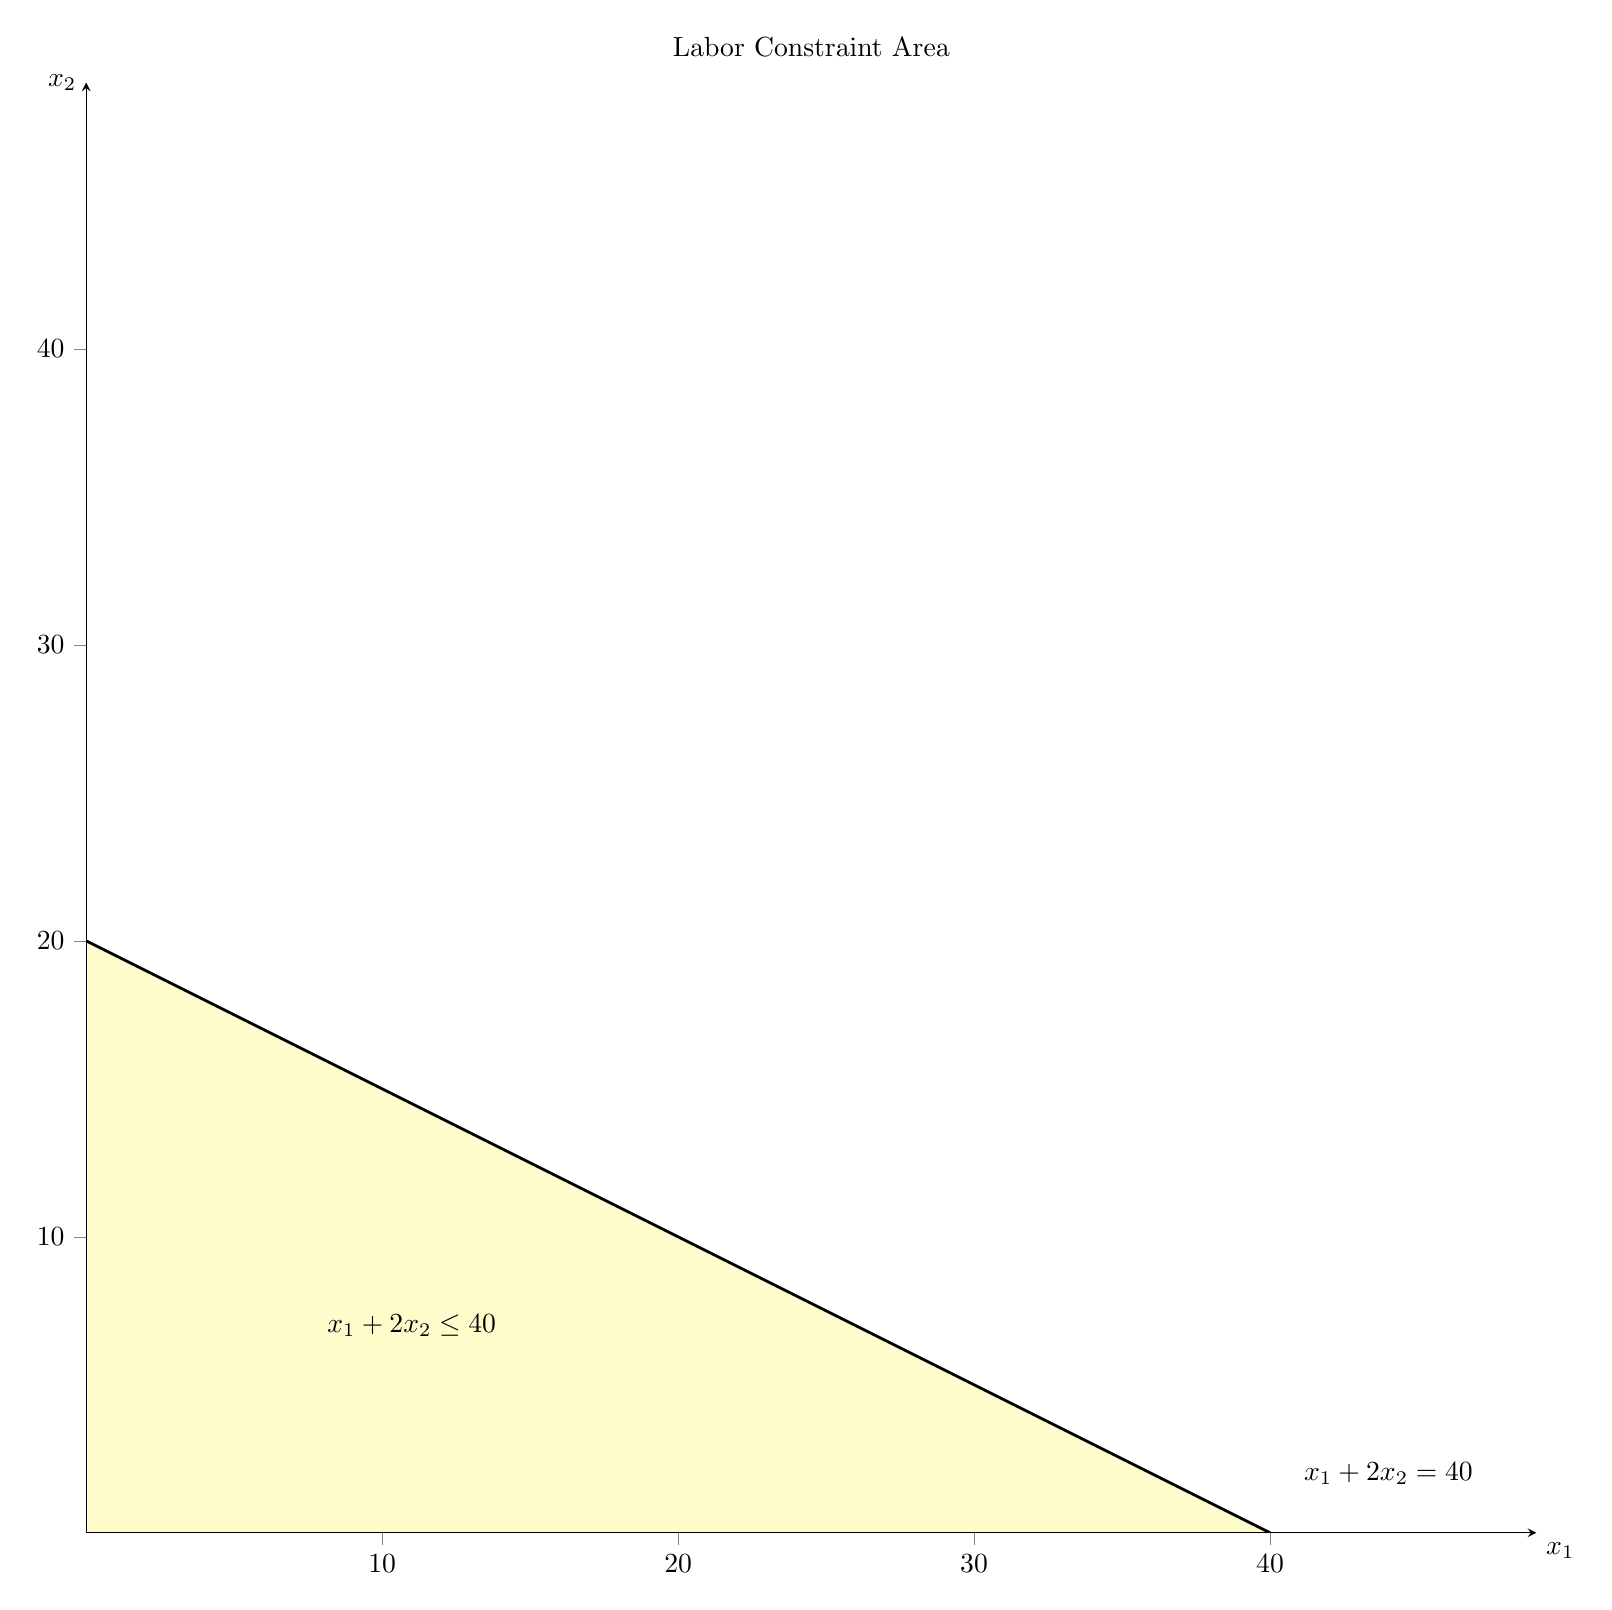
\begin{tikzpicture} [scale=1.0]
  \begin{axis}[
    name = plot1,
    title=Labor Constraint Area,
    width = 20cm, 
    height = 20cm,
    axis lines=left,
    axis equal image,
    axis on top = true, axis x line = middle, axis y line = middle,
    xmin = 0, ymin = 0, xmax = 49, ymax = 49,
    /pgfplots/xtick = {0,10,...,40},
    /pgfplots/ytick = {0,10,...,40},
    tick align = outside,
    xlabel = {$x_1$}, xlabel style = {at={(ticklabel* cs:1)},anchor = north west},
    ylabel = {$x_2$}, ylabel style = {at={(ticklabel* cs:1)},anchor = east},
    ]
    \path[name path=Zero]
      (\pgfkeysvalueof{/pgfplots/xmin},0) --
      (\pgfkeysvalueof{/pgfplots/xmax},0);

	\addplot[black,sharp plot, name path=Constraint1, line width = 1] coordinates {(0,20)(40,0)}; % 1
	\node at (44,2) {$x_1 + 2x_2 = 40$};

	\addplot[yellow!20] fill between[of=Constraint1 and Zero,soft clip={domain=0:40}];
	\node at (11,7) {$x_1 + 2x_2 \leq 40$};	
  \end{axis}
\end{tikzpicture}

% ------------------------------------------------------------------------------------------------------------------------

% ------------------------------------------------------------------------------------------------------------------------
% CLAY CONSTRAINT LINE
% ------------------------------------------------------------------------------------------------------------------------

\begin{tikzpicture} [scale=1.0]
  \begin{axis}[
    name = plot1,
    title=Clay Constraint Line,
    width = 20cm, 
    height = 20cm,
    axis lines=left,
    axis equal image,
    axis on top = true, axis x line = middle, axis y line = middle,
    xmin = 0, ymin = 0, xmax = 49, ymax = 49,
    /pgfplots/xtick = {0,10,...,40},
    /pgfplots/ytick = {0,10,...,40},
    tick align = outside,
    xlabel = {$x_1$}, xlabel style = {at={(ticklabel* cs:1)},anchor = north west},
    ylabel = {$x_2$}, ylabel style = {at={(ticklabel* cs:1)},anchor = east},
    ]
    \addplot[black,sharp plot, name path=Constraint2, line width = 1] coordinates {(0,40)(30,0)}; % 2
    \node at (6,40) {$4x_1 + 3x_2 = 120$};
  \end{axis}
\end{tikzpicture}

% ------------------------------------------------------------------------------------------------------------------------

% ------------------------------------------------------------------------------------------------------------------------
% CLAY CONSTRAINT SOLUTION AREA
% ------------------------------------------------------------------------------------------------------------------------

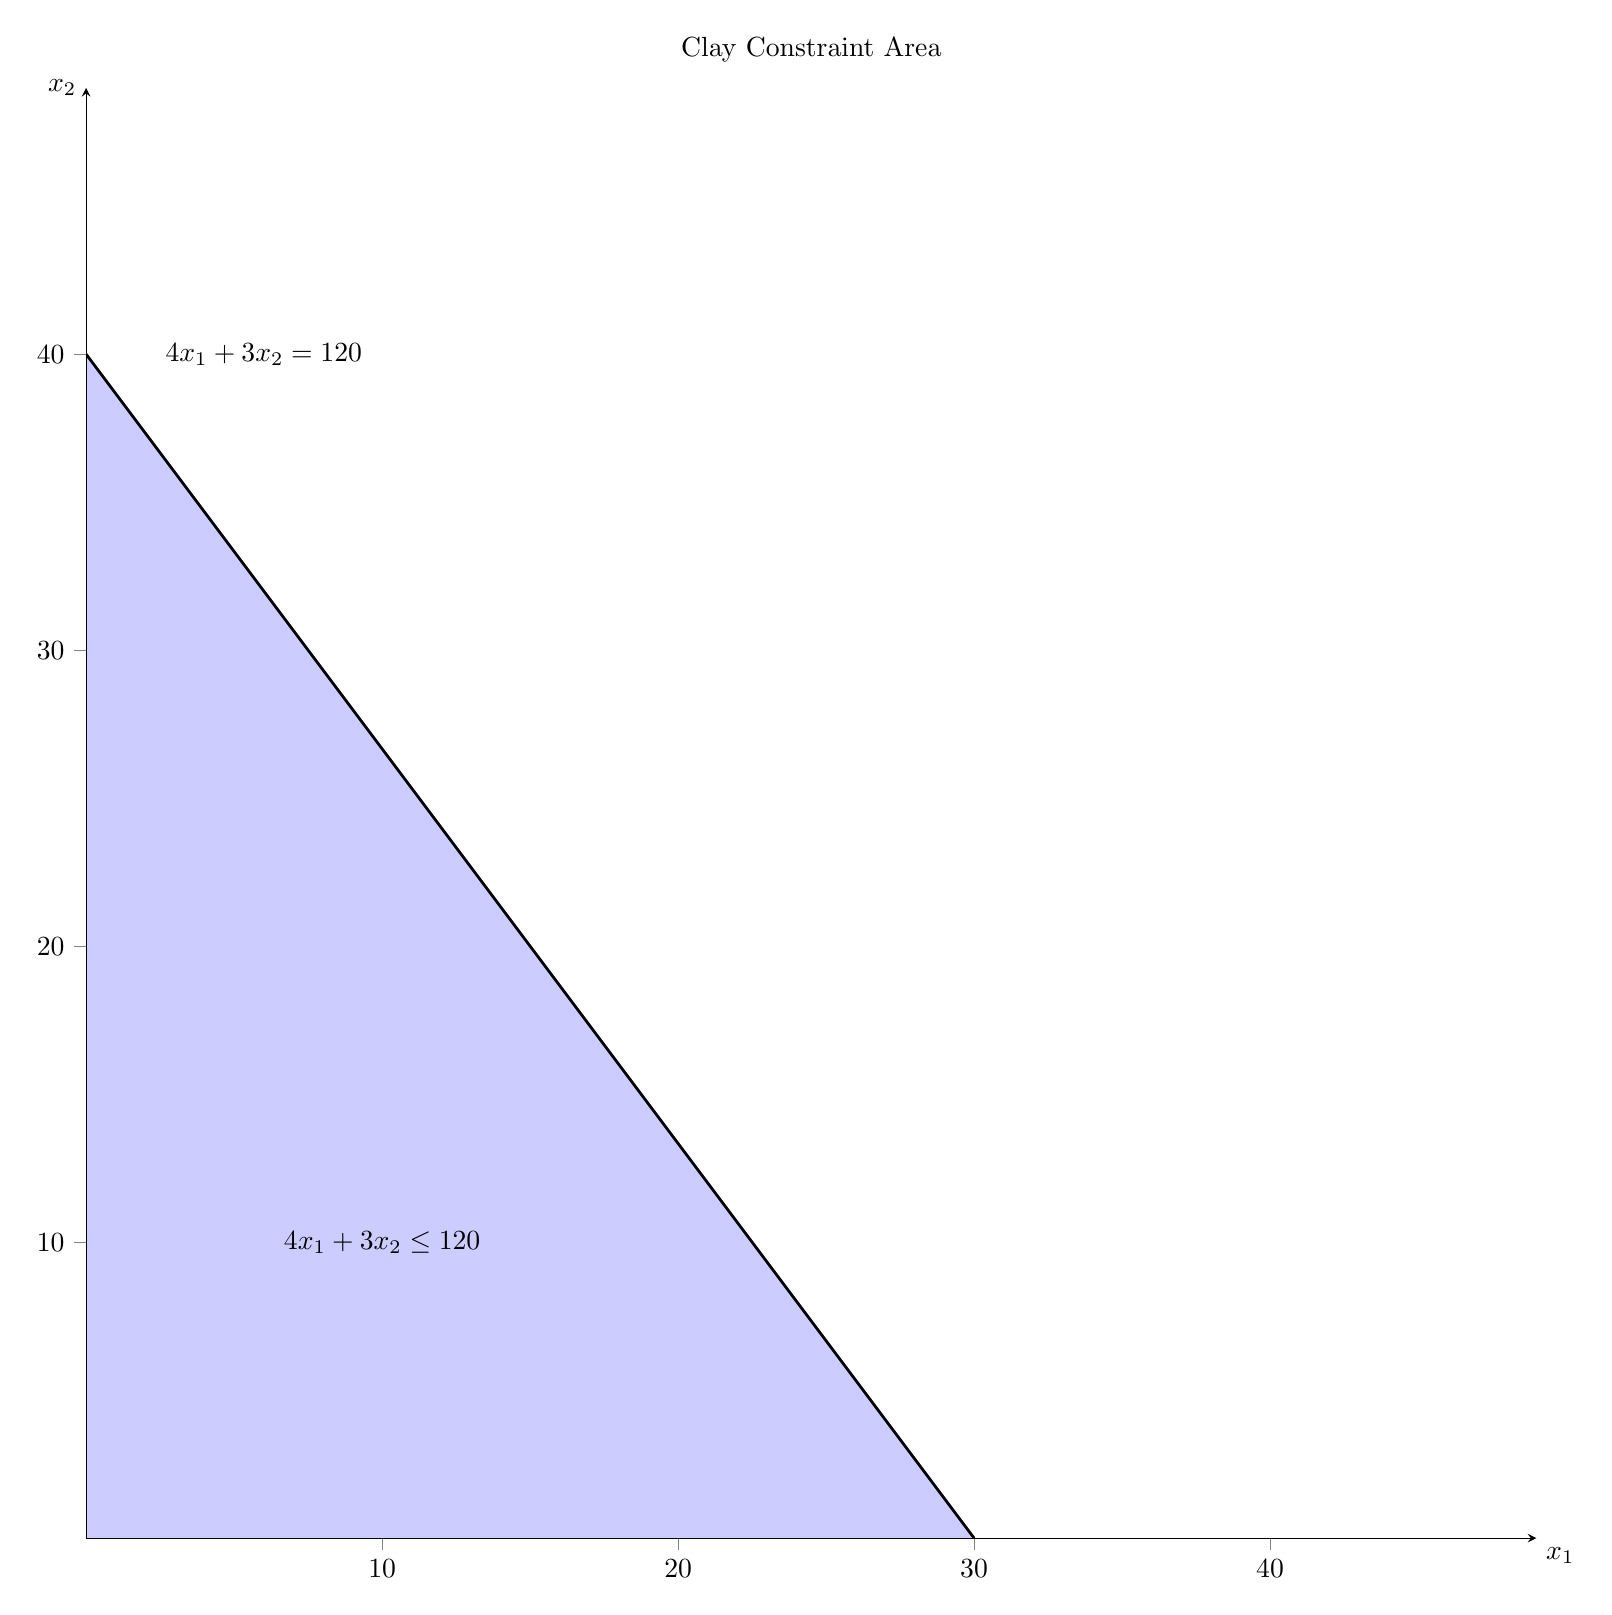
\begin{tikzpicture} [scale=1.0]
  \begin{axis}[
    name = plot1,
    title=Clay Constraint Area,
    width = 20cm, 
    height = 20cm,
    axis lines=left,
    axis equal image,
    axis on top = true, axis x line = middle, axis y line = middle,
    xmin = 0, ymin = 0, xmax = 49, ymax = 49,
    /pgfplots/xtick = {0,10,...,40},
    /pgfplots/ytick = {0,10,...,40},
    tick align = outside,
    xlabel = {$x_1$}, xlabel style = {at={(ticklabel* cs:1)},anchor = north west},
    ylabel = {$x_2$}, ylabel style = {at={(ticklabel* cs:1)},anchor = east},
    ]
    \path[name path=Zero]
      (\pgfkeysvalueof{/pgfplots/xmin},0) --
      (\pgfkeysvalueof{/pgfplots/xmax},0);

    \addplot[black,sharp plot, name path=Constraint2, line width = 1] coordinates {(0,40)(30,0)}; % 2
    \node at (6,40) {$4x_1 + 3x_2 = 120$};

	\addplot[blue!20] fill between[of=Constraint2 and Zero,soft clip={domain=0:30}];
    \node at (10,10) {$4x_1 + 3x_2 \leq 120$};
  \end{axis}
\end{tikzpicture}

% ------------------------------------------------------------------------------------------------------------------------

% ------------------------------------------------------------------------------------------------------------------------
% AREA OF TWO CONSTRAINTS
% ------------------------------------------------------------------------------------------------------------------------

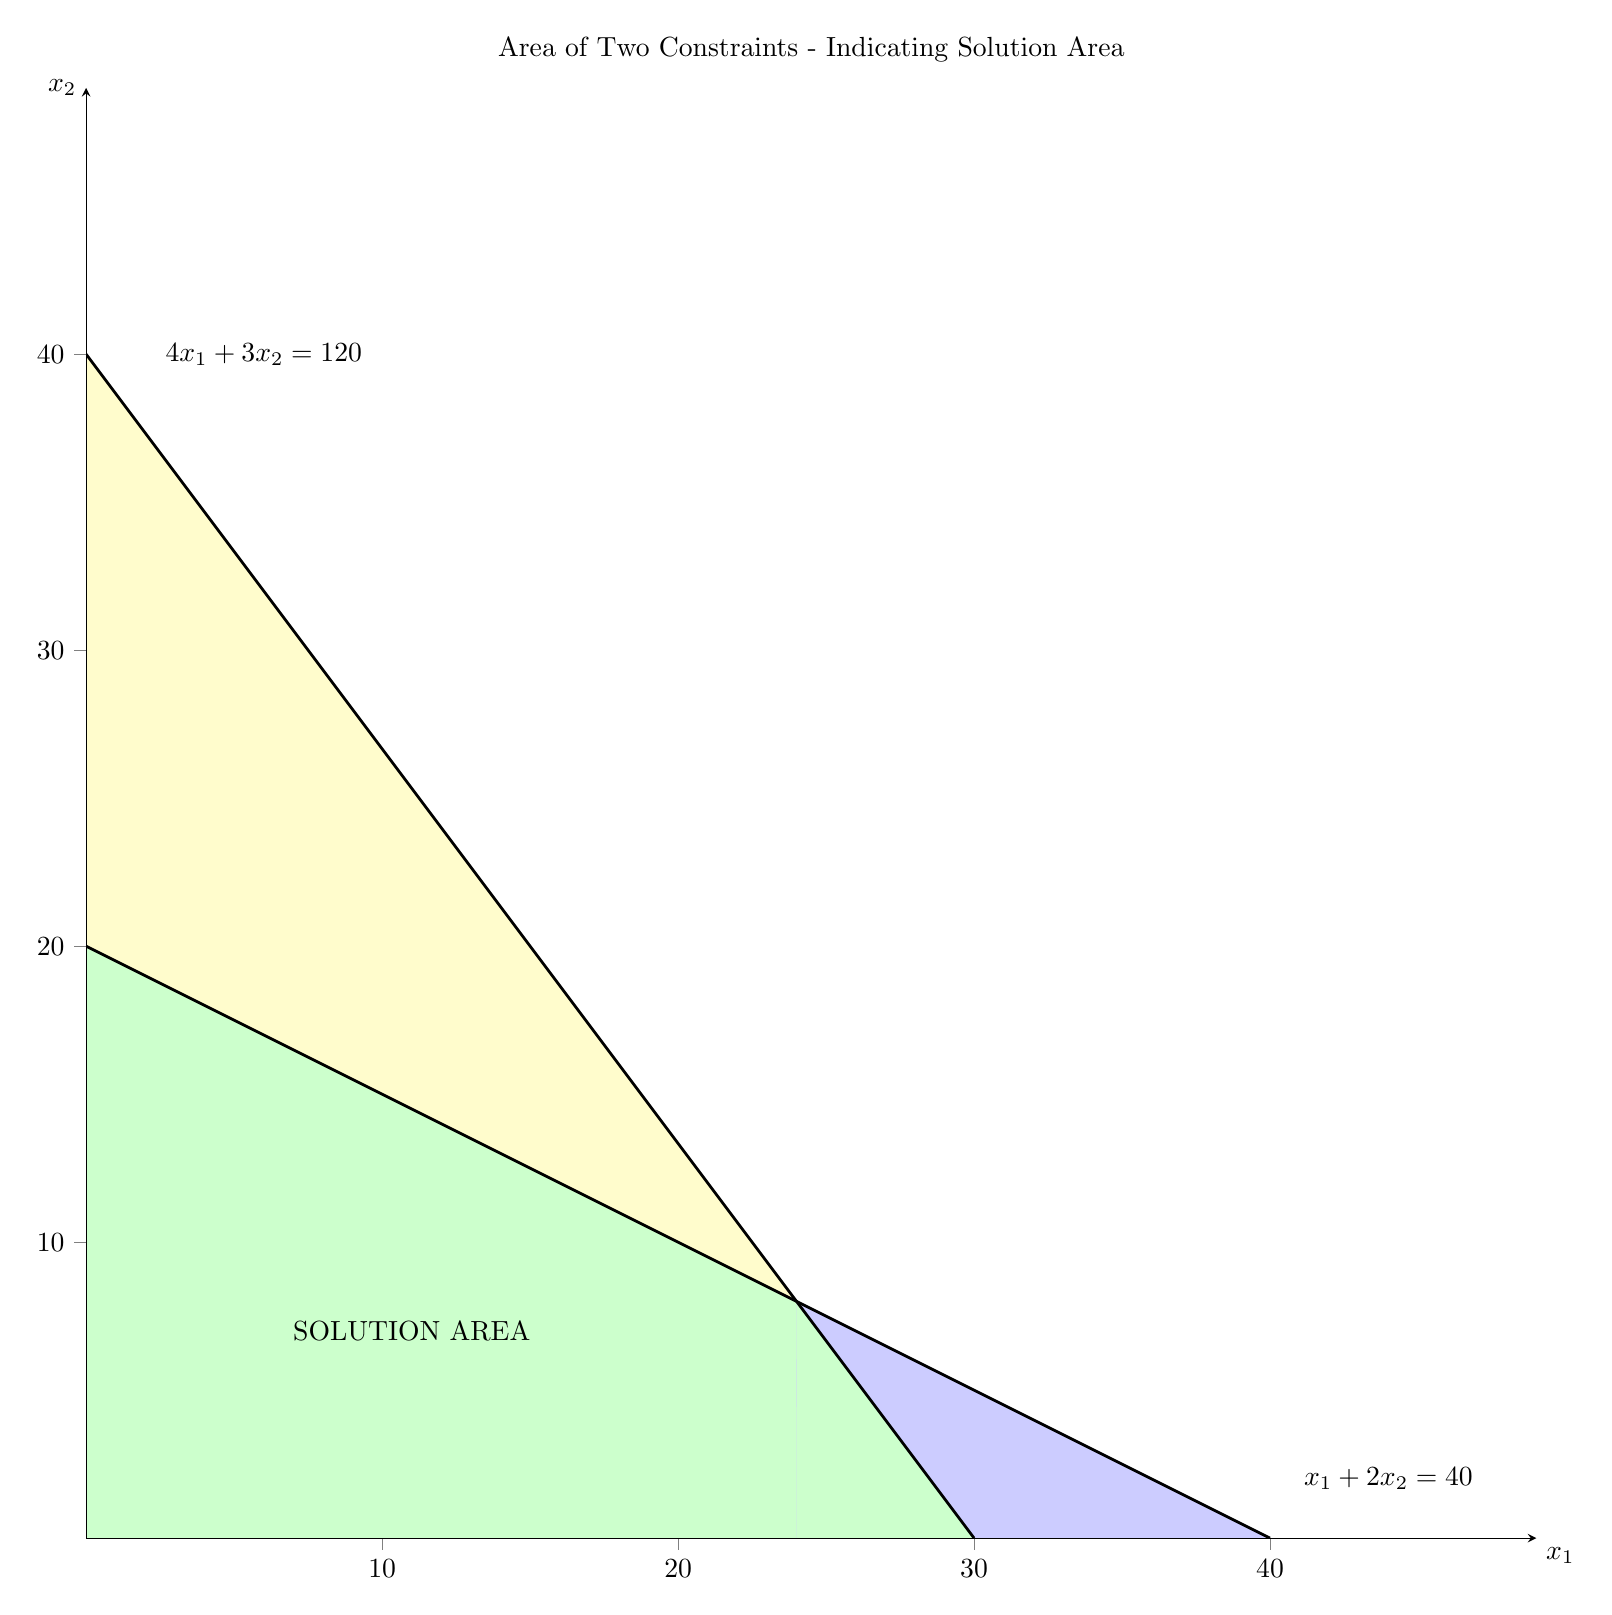
\begin{tikzpicture} [scale=1.0]
  \begin{axis}[
    name = plot1,
    title=Area of Two Constraints - Indicating Solution Area,
    width = 20cm, 
    height = 20cm,
    axis lines=left,
    axis equal image,
    axis on top = true, axis x line = middle, axis y line = middle,
    xmin = 0, ymin = 0, xmax = 49, ymax = 49,
    /pgfplots/xtick = {0,10,...,40},
    /pgfplots/ytick = {0,10,...,40},
    tick align = outside,
    xlabel = {$x_1$}, xlabel style = {at={(ticklabel* cs:1)},anchor = north west},
    ylabel = {$x_2$}, ylabel style = {at={(ticklabel* cs:1)},anchor = east},
    ]
    \path[name path=Zero]
      (\pgfkeysvalueof{/pgfplots/xmin},0) --
      (\pgfkeysvalueof{/pgfplots/xmax},0);

    \addplot[black,sharp plot, name path=Constraint2, line width = 1] coordinates {(0,40)(30,0)}; % 2
    \node at (6,40) {$4x_1 + 3x_2 = 120$};
	\addplot[yellow!20] fill between[of=Constraint2 and Zero,soft clip={domain=0:30}];

	\addplot[black,sharp plot, name path=Constraint1, line width = 1] coordinates {(0,20)(40,0)}; % 1
	\node at (44,2) {$x_1 + 2x_2 = 40$};
	\addplot[blue!20] fill between[of=Constraint1 and Zero,soft clip={domain=0:40}];

	%\addplot[black,sharp plot, line width = 2] coordinates {(0,0)(30,0)(24,8)(0,20)};
	\node at (11,7) {SOLUTION AREA};	

	\addplot[green!20] fill between[of=Constraint1 and Zero,soft clip={domain=0:24}];
	\addplot[green!20] fill between[of=Constraint2 and Zero,soft clip={domain=24:30}];
	
  \end{axis}
\end{tikzpicture}

% ------------------------------------------------------------------------------------------------------------------------

% ------------------------------------------------------------------------------------------------------------------------
% SOLUTION AREA
% ------------------------------------------------------------------------------------------------------------------------

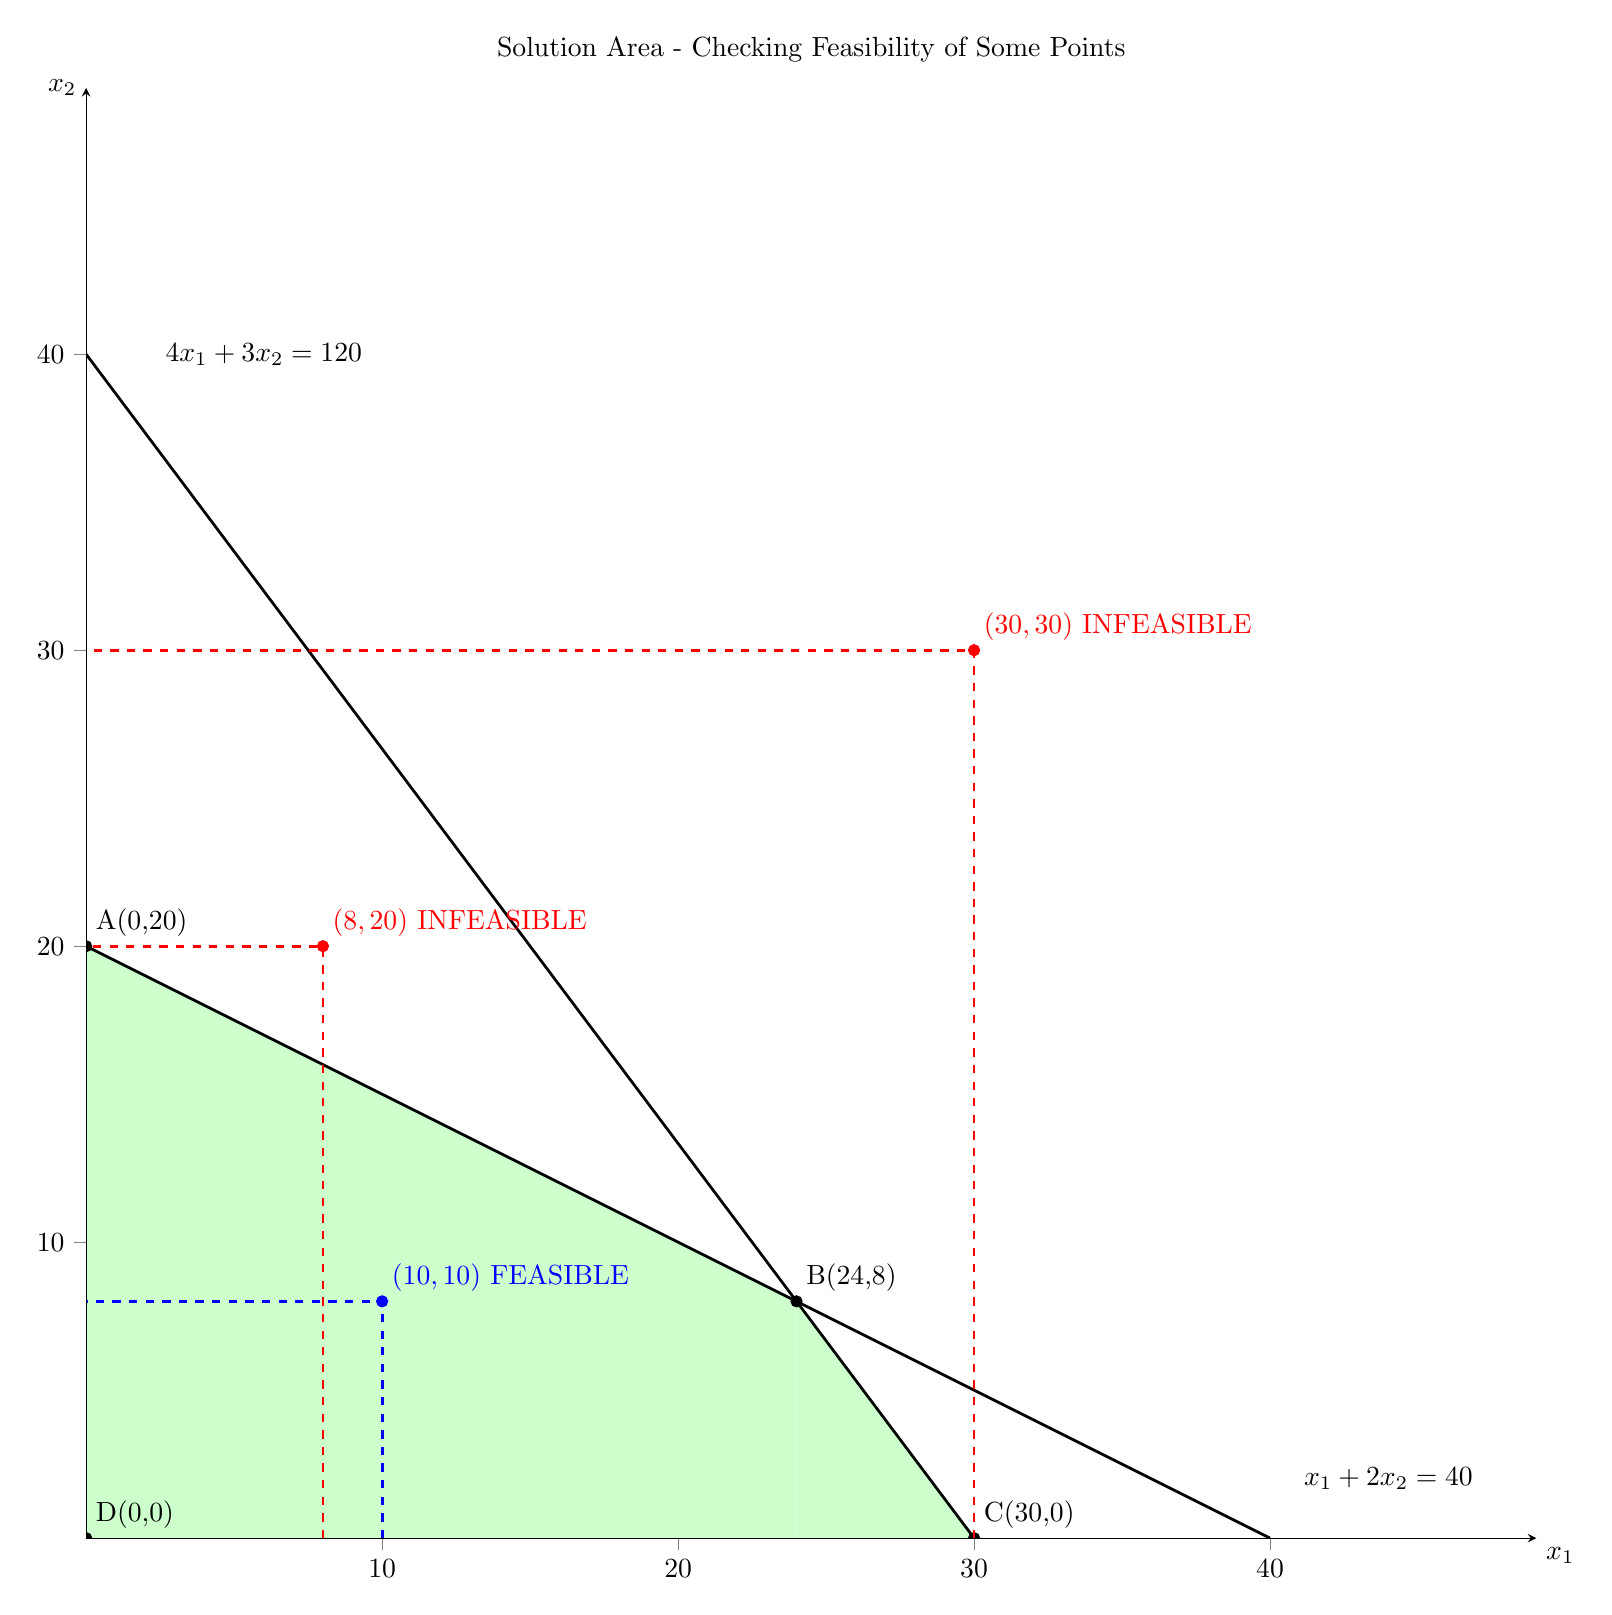
\begin{tikzpicture} [scale=1.0]
  \begin{axis}[
    name = plot1,
    title=Solution Area - Checking Feasibility of Some Points,
    width = 20cm, 
    height = 20cm,
    axis lines=left,
    axis equal image,
    axis on top = true, axis x line = middle, axis y line = middle,
    xmin = 0, ymin = 0, xmax = 49, ymax = 49,
    /pgfplots/xtick = {0,10,...,40},
    /pgfplots/ytick = {0,10,...,40},
    tick align = outside,
    xlabel = {$x_1$}, xlabel style = {at={(ticklabel* cs:1)},anchor = north west},
    ylabel = {$x_2$}, ylabel style = {at={(ticklabel* cs:1)},anchor = east},
    ]
    \path[name path=Zero]
      (\pgfkeysvalueof{/pgfplots/xmin},0) --
      (\pgfkeysvalueof{/pgfplots/xmax},0);

    \addplot[black,sharp plot, name path=Constraint2, line width = 1] coordinates {(0,40)(30,0)}; % 2
    \node at (6,40) {$4x_1 + 3x_2 = 120$};

	\addplot[black,sharp plot, name path=Constraint1, line width = 1] coordinates {(0,20)(40,0)}; % 1
	\node at (44,2) {$x_1 + 2x_2 = 40$};

	\addplot[green!20] fill between[of=Constraint1 and Zero,soft clip={domain=0:24}];
	\addplot[green!20] fill between[of=Constraint2 and Zero,soft clip={domain=24:30}];

    \filldraw[black] (0,20) circle (2pt) node[anchor=south west] {A(0,20)};
    \filldraw[black] (24,8) circle (2pt) node[anchor=south west] {B(24,8)};
    \filldraw[black] (30,0) circle (2pt) node[anchor=south west] {C(30,0)};
    \filldraw[black] (0,0) circle (2pt) node[anchor=south west] {D(0,0)};

	\addplot[blue,dashed, line width = 1] coordinates {(10,0)(10,8)(0,8)};
    \filldraw[blue] (10,8) circle (2pt) node[anchor=south west] {$(10,10)$ FEASIBLE};
	\addplot[red,dashed, line width = 1] coordinates {(8,0)(8,20)(0,20)};
    \filldraw[red] (8,20) circle (2pt) node[anchor=south west] {$(8,20)$ INFEASIBLE};
	\addplot[red,dashed, line width = 1] coordinates {(30,0)(30,30)(0,30)};
    \filldraw[red] (30,30) circle (2pt) node[anchor=south west] {$(30,30)$ INFEASIBLE};

	
  \end{axis}
\end{tikzpicture}

% ------------------------------------------------------------------------------------------------------------------------

% ------------------------------------------------------------------------------------------------------------------------
% OBJECTIVE FUNCTION FOR Z = 800
% ------------------------------------------------------------------------------------------------------------------------

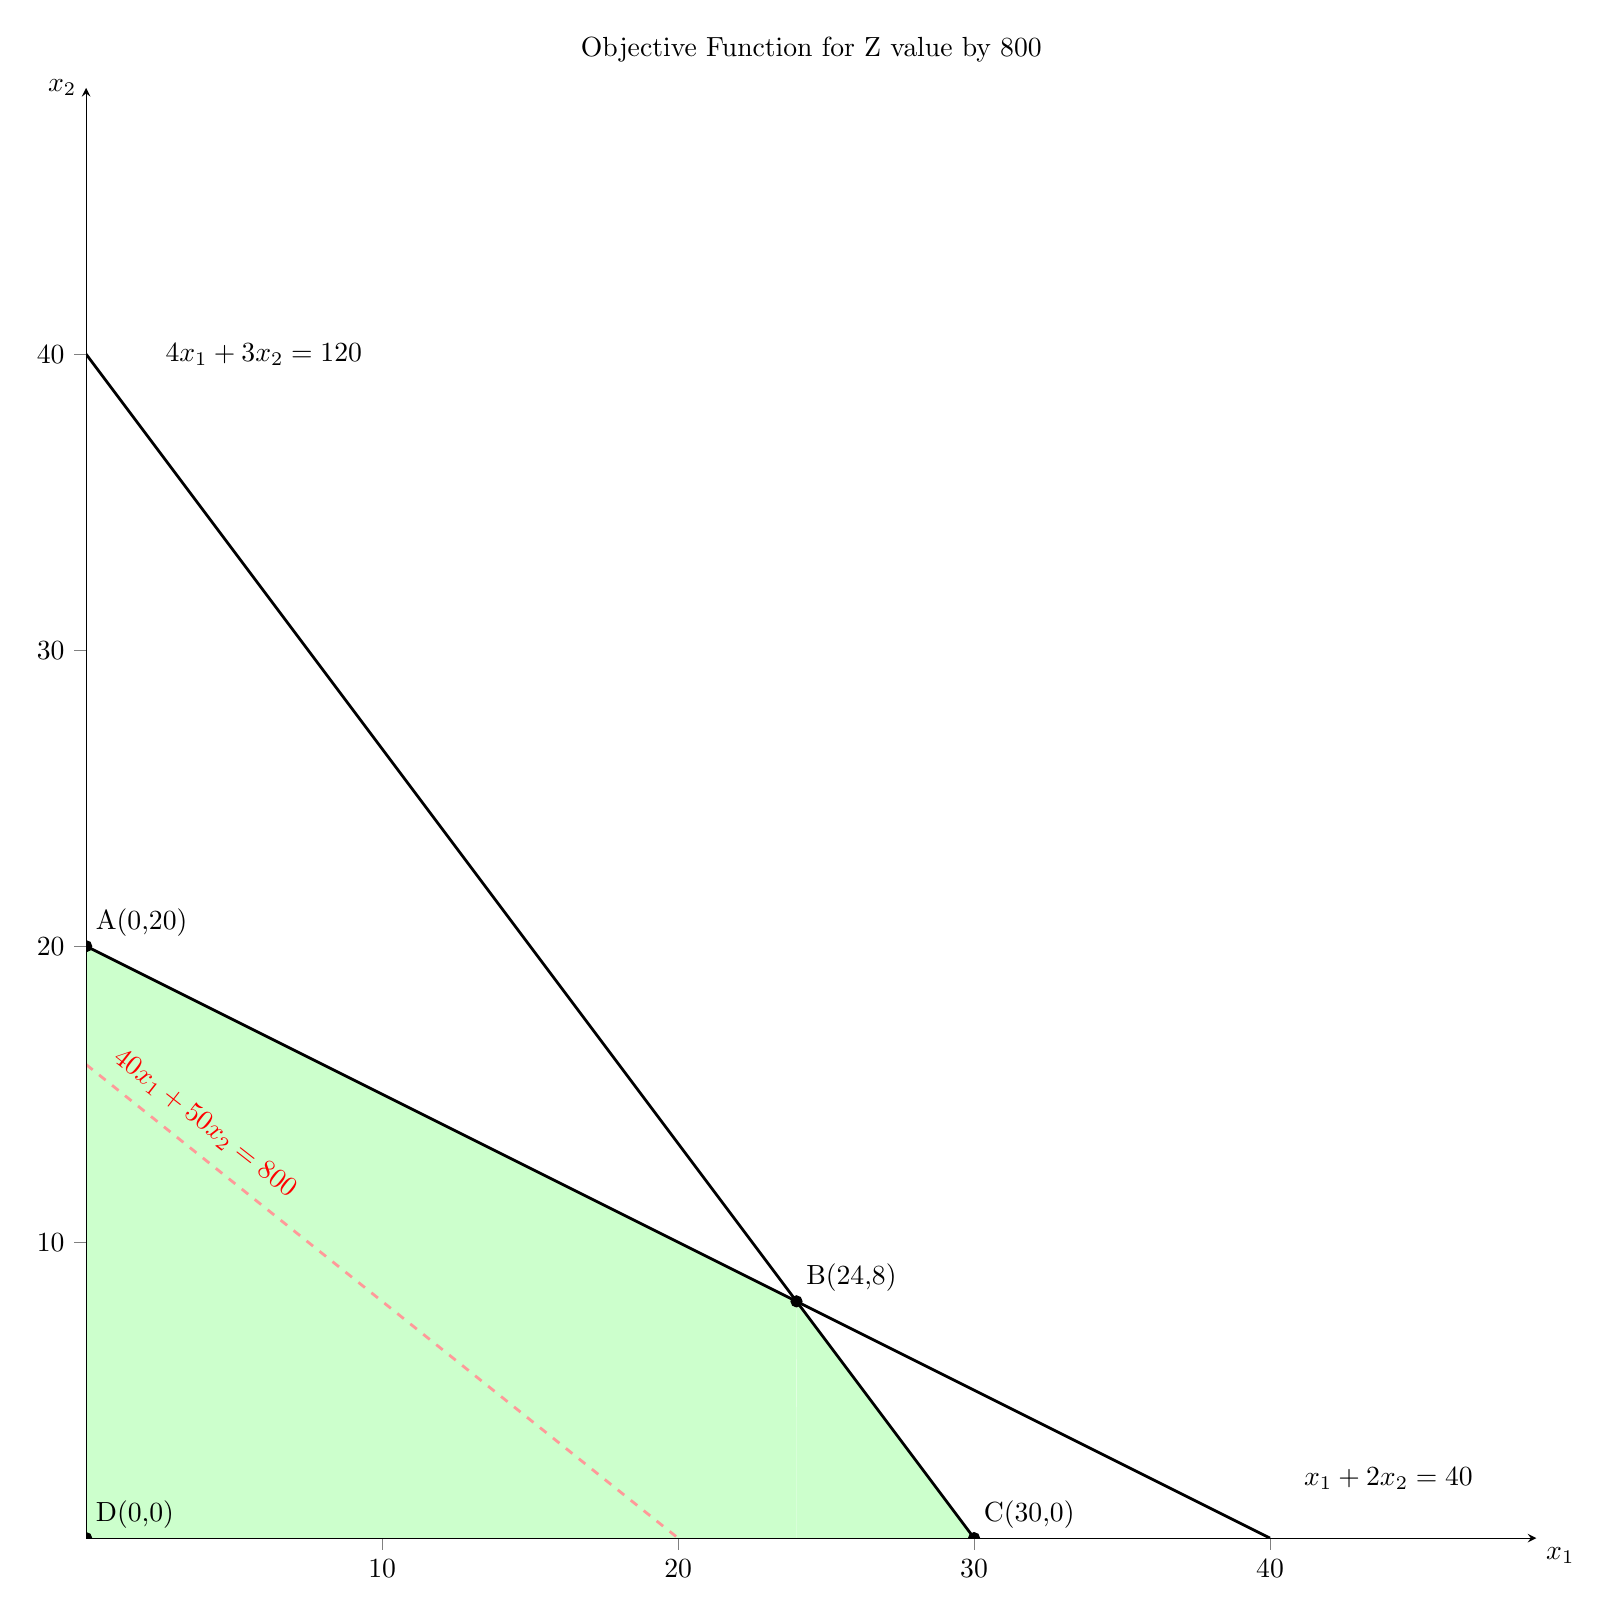
\begin{tikzpicture} [scale=1.0]
  \begin{axis}[
    name = plot1,
    title=Objective Function for Z value by 800,
    width = 20cm, 
    height = 20cm,
    axis lines=left,
    axis equal image,
    axis on top = true, axis x line = middle, axis y line = middle,
    xmin = 0, ymin = 0, xmax = 49, ymax = 49,
    /pgfplots/xtick = {0,10,...,40},
    /pgfplots/ytick = {0,10,...,40},
    tick align = outside,
    xlabel = {$x_1$}, xlabel style = {at={(ticklabel* cs:1)},anchor = north west},
    ylabel = {$x_2$}, ylabel style = {at={(ticklabel* cs:1)},anchor = east},
    ]
    \path[name path=Zero]
      (\pgfkeysvalueof{/pgfplots/xmin},0) --
      (\pgfkeysvalueof{/pgfplots/xmax},0);

    \addplot[black,sharp plot, name path=Constraint2, line width = 1] coordinates {(0,40)(30,0)}; % 2
    \node at (6,40) {$4x_1 + 3x_2 = 120$};

	\addplot[black,sharp plot, name path=Constraint1, line width = 1] coordinates {(0,20)(40,0)}; % 1
	\node at (44,2) {$x_1 + 2x_2 = 40$};

	\addplot[green!20] fill between[of=Constraint1 and Zero,soft clip={domain=0:24}];
	\addplot[green!20] fill between[of=Constraint2 and Zero,soft clip={domain=24:30}];

    \filldraw[black] (0,20) circle (2pt) node[anchor=south west] {A(0,20)};
    \filldraw[black] (24,8) circle (2pt) node[anchor=south west] {B(24,8)};
    \filldraw[black] (30,0) circle (2pt) node[anchor=south west] {C(30,0)};
    \filldraw[black] (0,0) circle (2pt) node[anchor=south west] {D(0,0)};

    \addplot[red!40,dashed, name path=Objective2, line width = 1] coordinates {(0,16)(20,0)};
   	\node [rotate=-38,red] at (4,14) {$40x_1 + 50x_2 = 800$};
  \end{axis}
\end{tikzpicture}

% ------------------------------------------------------------------------------------------------------------------------

% ------------------------------------------------------------------------------------------------------------------------
% OBJECTIVE FUNCTION FOR Z = 800, 1200 AND 1600
% ------------------------------------------------------------------------------------------------------------------------

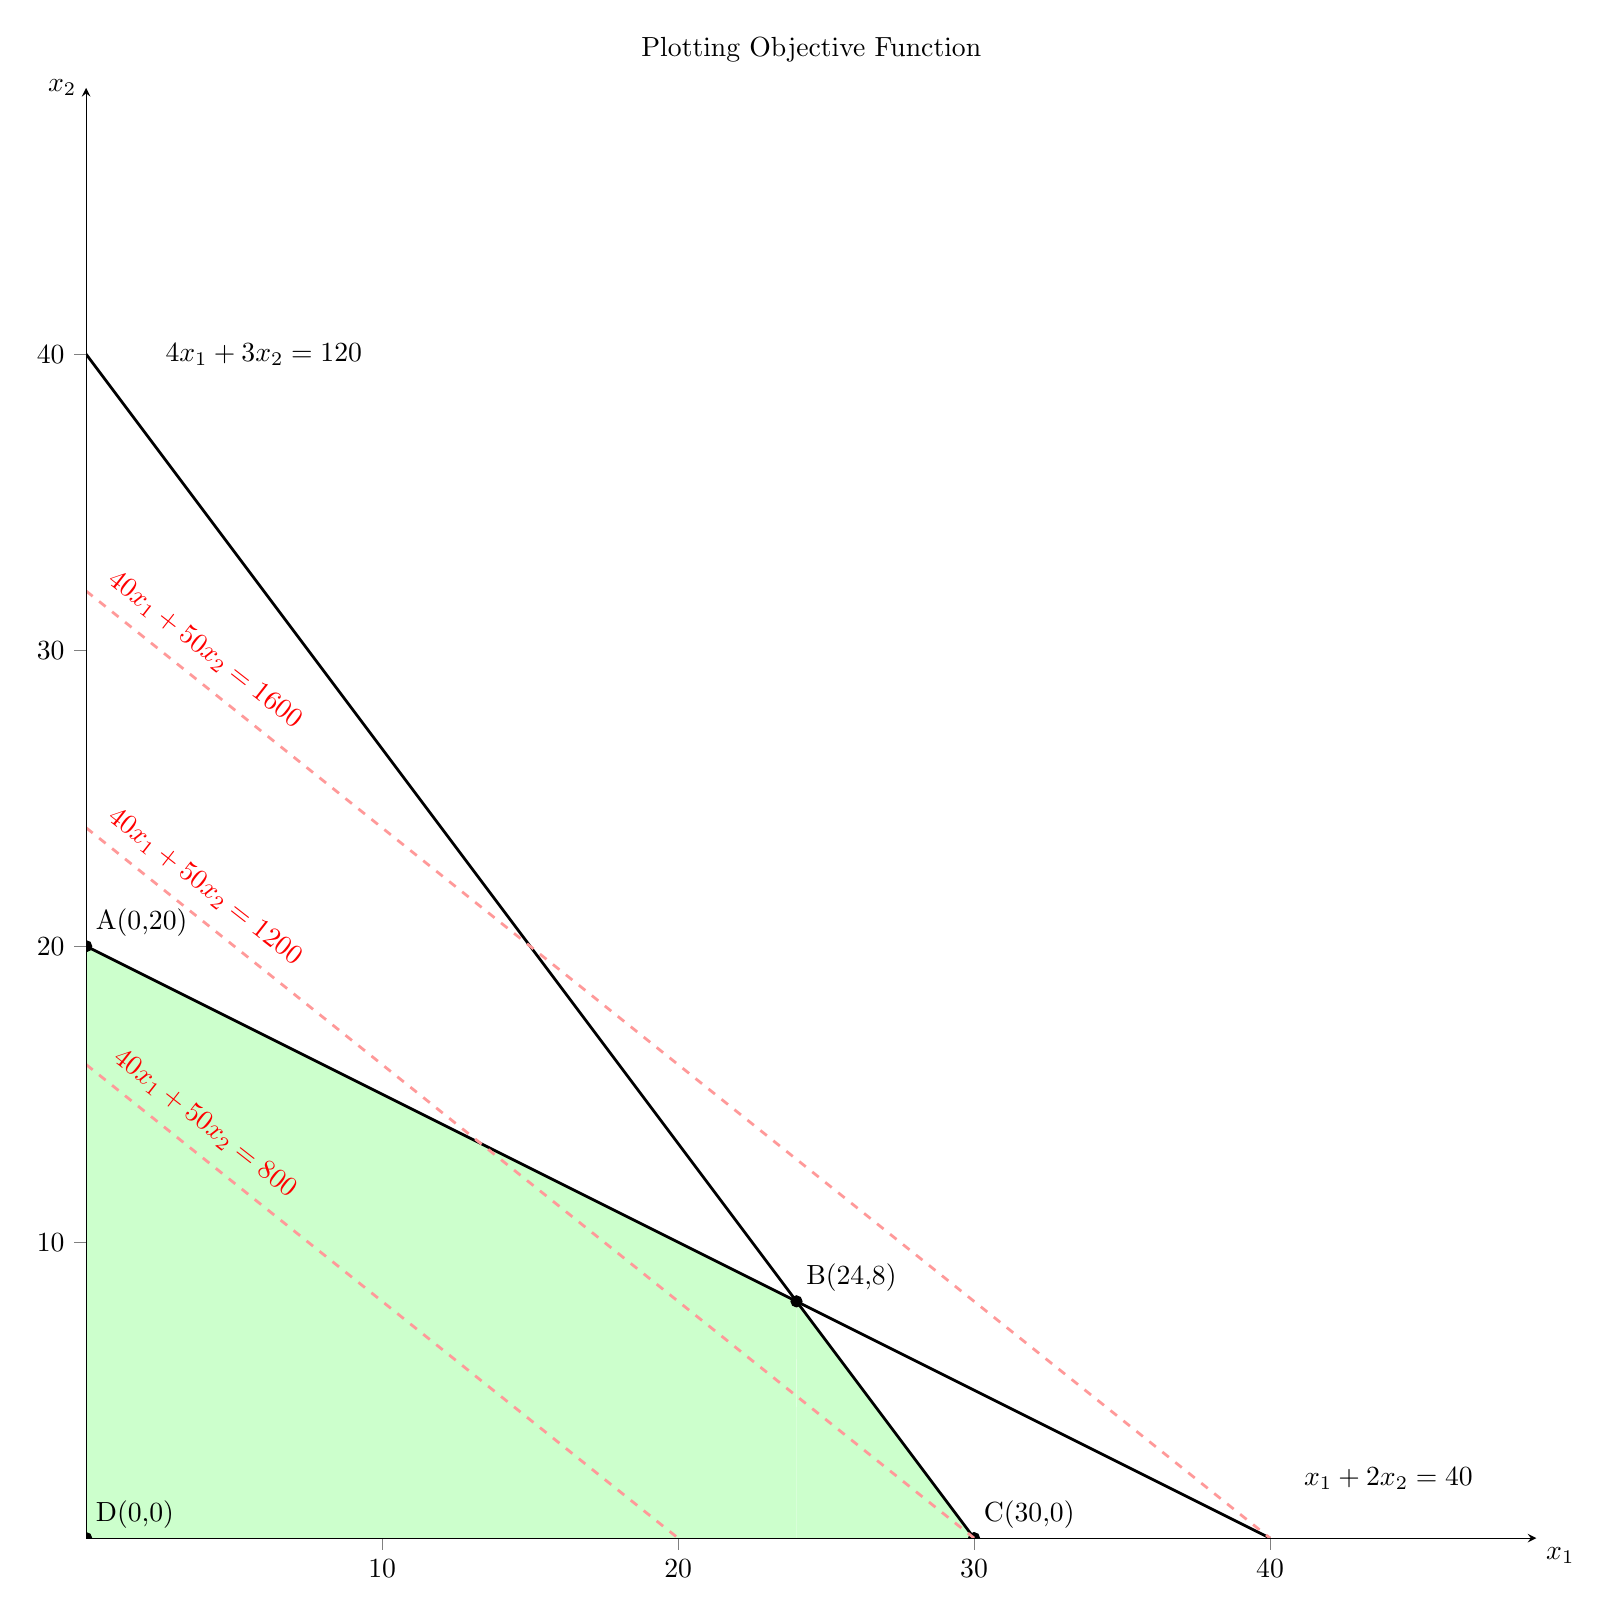
\begin{tikzpicture} [scale=1.0]
  \begin{axis}[
    name = plot1,
    title=Plotting Objective Function,
    width = 20cm, 
    height = 20cm,
    axis lines=left,
    axis equal image,
    axis on top = true, axis x line = middle, axis y line = middle,
    xmin = 0, ymin = 0, xmax = 49, ymax = 49,
    /pgfplots/xtick = {0,10,...,40},
    /pgfplots/ytick = {0,10,...,40},
    tick align = outside,
    xlabel = {$x_1$}, xlabel style = {at={(ticklabel* cs:1)},anchor = north west},
    ylabel = {$x_2$}, ylabel style = {at={(ticklabel* cs:1)},anchor = east},
    ]
    \path[name path=Zero]
      (\pgfkeysvalueof{/pgfplots/xmin},0) --
      (\pgfkeysvalueof{/pgfplots/xmax},0);

    \addplot[black,sharp plot, name path=Constraint2, line width = 1] coordinates {(0,40)(30,0)}; % 2
    \node at (6,40) {$4x_1 + 3x_2 = 120$};

	\addplot[black,sharp plot, name path=Constraint1, line width = 1] coordinates {(0,20)(40,0)}; % 1
	\node at (44,2) {$x_1 + 2x_2 = 40$};

	\addplot[green!20] fill between[of=Constraint1 and Zero,soft clip={domain=0:24}];
	\addplot[green!20] fill between[of=Constraint2 and Zero,soft clip={domain=24:30}];

    \filldraw[black] (0,20) circle (2pt) node[anchor=south west] {A(0,20)};
    \filldraw[black] (24,8) circle (2pt) node[anchor=south west] {B(24,8)};
    \filldraw[black] (30,0) circle (2pt) node[anchor=south west] {C(30,0)};
    \filldraw[black] (0,0) circle (2pt) node[anchor=south west] {D(0,0)};

    \addplot[red!40,dashed, name path=Objective2, line width = 1] coordinates {(0,16)(20,0)};
   	\node [rotate=-38,red] at (4,14) {$40x_1 + 50x_2 = 800$};
	\addplot[red!40,dashed, name path=Objective3, line width = 1] coordinates {(0,24)(30,0)};
   	\node [rotate=-38,red] at (4,22) {$40x_1 + 50x_2 = 1200$};
    \addplot[red!40,dashed, name path=Objective4, line width = 1] coordinates {(0,32)(40,0)};
   	\node [rotate=-38,red] at (4,30) {$40x_1 + 50x_2 = 1600$};    
  \end{axis}
\end{tikzpicture}

% ------------------------------------------------------------------------------------------------------------------------

% ------------------------------------------------------------------------------------------------------------------------
% OBJECTIVE FUNCTION FOR Z = 1360
% ------------------------------------------------------------------------------------------------------------------------

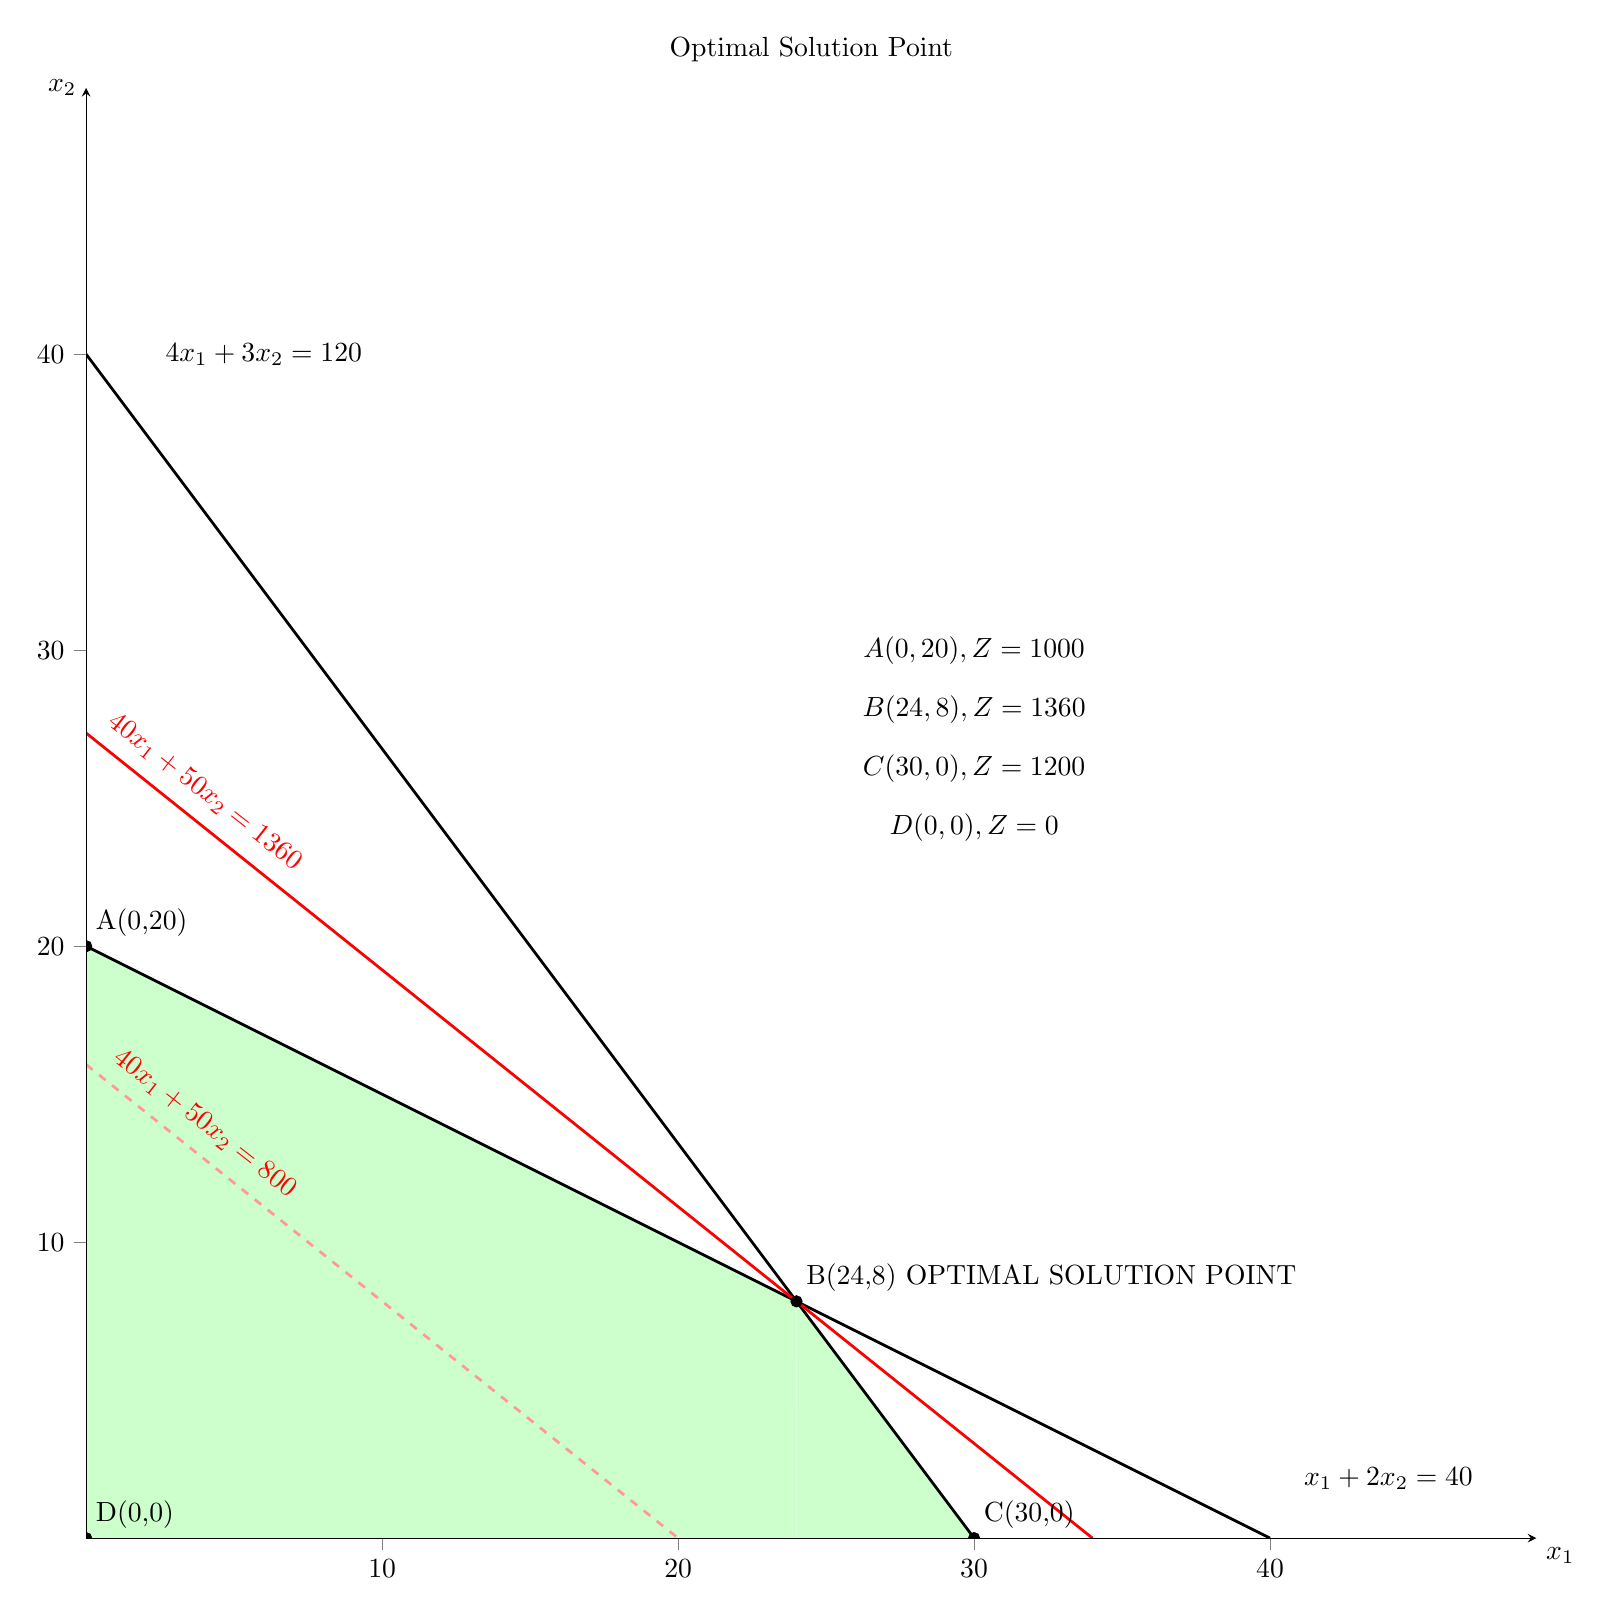
\begin{tikzpicture} [scale=1.0]
  \begin{axis}[
    name = plot1,
    title=Optimal Solution Point,
    width = 20cm, 
    height = 20cm,
    axis lines=left,
    axis equal image,
    axis on top = true, axis x line = middle, axis y line = middle,
    xmin = 0, ymin = 0, xmax = 49, ymax = 49,
    /pgfplots/xtick = {0,10,...,40},
    /pgfplots/ytick = {0,10,...,40},
    tick align = outside,
    xlabel = {$x_1$}, xlabel style = {at={(ticklabel* cs:1)},anchor = north west},
    ylabel = {$x_2$}, ylabel style = {at={(ticklabel* cs:1)},anchor = east},
    ]
    \path[name path=Zero]
      (\pgfkeysvalueof{/pgfplots/xmin},0) --
      (\pgfkeysvalueof{/pgfplots/xmax},0);

    \addplot[black,sharp plot, name path=Constraint2, line width = 1] coordinates {(0,40)(30,0)}; % 2
    \node at (6,40) {$4x_1 + 3x_2 = 120$};

	\addplot[black,sharp plot, name path=Constraint1, line width = 1] coordinates {(0,20)(40,0)}; % 1
	\node at (44,2) {$x_1 + 2x_2 = 40$};

	\addplot[green!20] fill between[of=Constraint1 and Zero,soft clip={domain=0:24}];
	\addplot[green!20] fill between[of=Constraint2 and Zero,soft clip={domain=24:30}];

    \addplot[red!40,dashed, name path=Objective2, line width = 1] coordinates {(0,16)(20,0)};
   	\node [rotate=-38,red] at (4,14) {$40x_1 + 50x_2 = 800$};

    \addplot[red,sharp plot, name path=ObjectiveA, line width = 1] coordinates {(0,27.2)(34,0)}; % Objective function A
   	\node [rotate=-38,red] at (4,25.2) {$40x_1 + 50x_2 = 1360$};

    \filldraw[black] (0,20) circle (2pt) node[anchor=south west] {A(0,20)};
    \filldraw[black] (24,8) circle (2pt) node[anchor=south west] {B(24,8) OPTIMAL SOLUTION POINT};
    \filldraw[black] (30,0) circle (2pt) node[anchor=south west] {C(30,0)};
    \filldraw[black] (0,0) circle (2pt) node[anchor=south west] {D(0,0)};

    \node at (30,30) {$A(0,20), Z = 1000$};
    \node at (30,28) {$B(24,8), Z = 1360$};
    \node at (30,26) {$C(30,0), Z = 1200$};
    \node at (30,24) {$D(0,0), Z = 0$}; 

  \end{axis}
\end{tikzpicture}

% ------------------------------------------------------------------------------------------------------------------------

% ------------------------------------------------------------------------------------------------------------------------
% OBJECTIVE FUNCTION FOR Z = 70 x_{1} + 20 x_{2} - THE MAIN GRAPH
% ------------------------------------------------------------------------------------------------------------------------

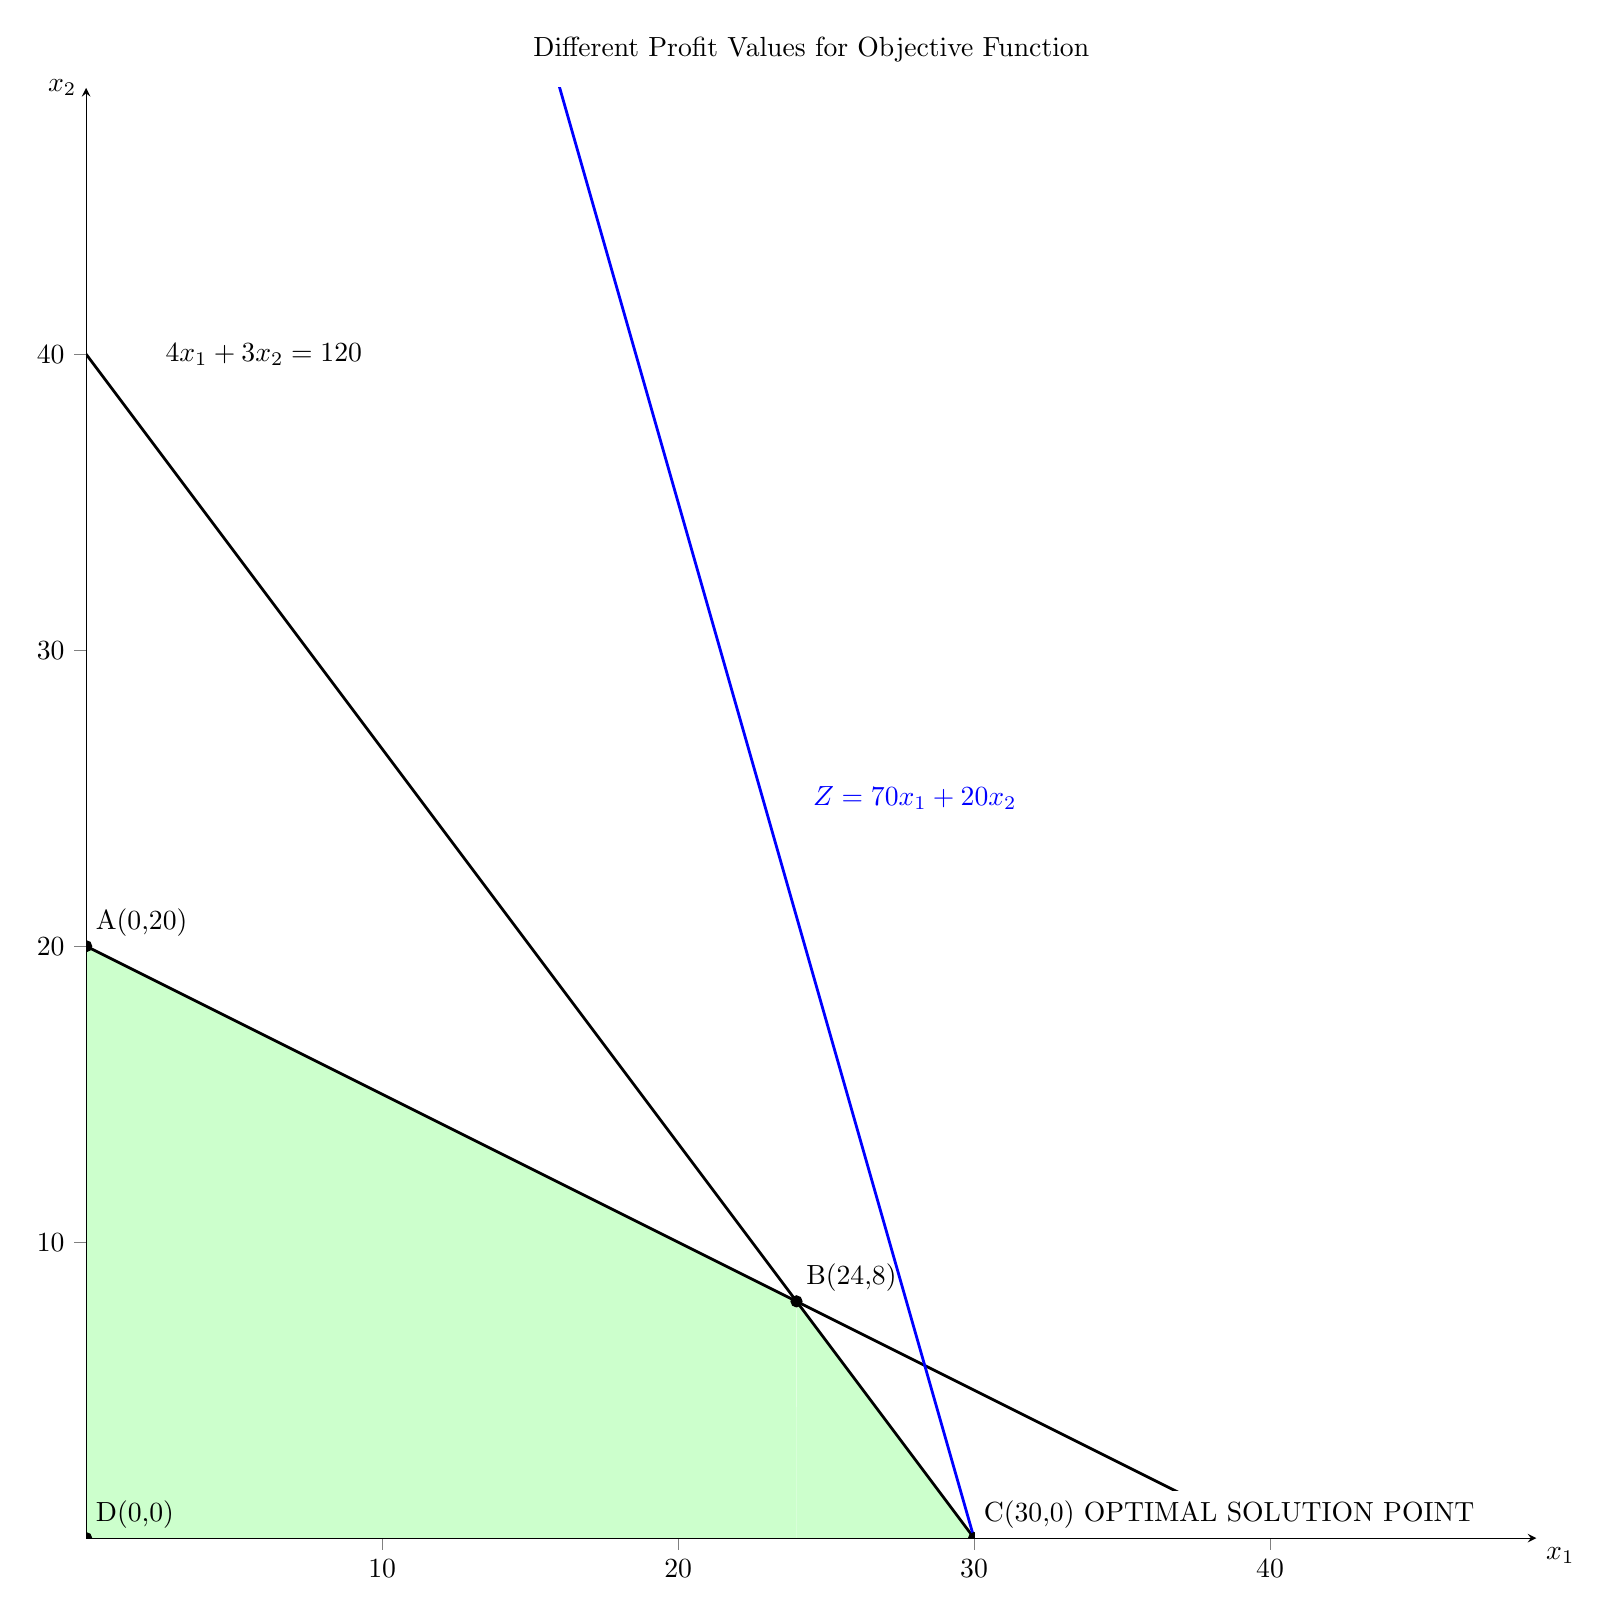
\begin{tikzpicture} [scale=1.0]
  \begin{axis}[
    name = plot1,
    title=Different Profit Values for Objective Function,
    width = 20cm, 
    height = 20cm,
    axis lines=left,
    axis equal image,
    axis on top = true, axis x line = middle, axis y line = middle,
    xmin = 0, ymin = 0, xmax = 49, ymax = 49,
    /pgfplots/xtick = {0,10,...,40},
    /pgfplots/ytick = {0,10,...,40},
    tick align = outside,
    xlabel = {$x_1$}, xlabel style = {at={(ticklabel* cs:1)},anchor = north west},
    ylabel = {$x_2$}, ylabel style = {at={(ticklabel* cs:1)},anchor = east},
    %legend entries={Constraint 1,Constraint 2,Constraint 3},
    ]
    %\addplot+[name path=Constraint1,red, line width = 1] coordinates {(0,50)(50,0)} node {$A$};
    %\addplot+[name path=Constraint1, line width = 1] coordinates {(0,50)(50,0)} node[pin=45:{B}]{};
    \path[name path=Zero]
      (\pgfkeysvalueof{/pgfplots/xmin},0) --
      (\pgfkeysvalueof{/pgfplots/xmax},0);
    \addplot[black,sharp plot, name path=Constraint1, line width = 1] coordinates {(0,20)(40,0)}; % 1
    \addplot[black,sharp plot, name path=Constraint2, line width = 1] coordinates {(0,40)(30,0)}; % 2
%    \node at (44,2) {$x_1 + 2x_2 = 40$};
    \node at (6,40) {$4x_1 + 3x_2 = 120$};
    \node [blue] at (28,25) {$Z = 70x_1 + 20x_2$};

%    \addplot[red!40,dashed, name path=Objective1, line width = 1] coordinates {(0,8)(10,0)};
%    \addplot[red!40,dashed, name path=Objective2, line width = 1] coordinates {(0,16)(20,0)};
%    \addplot[red!40,dashed, name path=Objective3, line width = 1] coordinates {(0,24)(30,0)};
%    \addplot[red!40,dashed, name path=Objective4, line width = 1] coordinates {(0,32)(40,0)};
%    \addplot[red,sharp plot, name path=ObjectiveA, line width = 1] coordinates {(0,27.2)(34,0)}; % Objective function A
    \addplot[blue,sharp plot, name path=ObjectiveB, line width = 1] coordinates {(0,105)(30,0)}; % Objective function B
%    \addplot[green,sharp plot, name path=ObjectiveC, line width = 1] coordinates {(0,20)(70,0)}; % Objective function C
        
    %\addplot[green!20] fill between[of=Constraint1 and Zero,soft clip={domain=0:40}];
    %\addplot[fill opacity=0.50,blue!40] fill between[of=Constraint2 and Zero];

    \filldraw[black] (0,20) circle (2pt) node[anchor=south west] {A(0,20)};
    \filldraw[black] (24,8) circle (2pt) node[anchor=south west] {B(24,8)};
    \filldraw[black] (30,0) circle (2pt) node[anchor=south west,fill=white] {C(30,0) OPTIMAL SOLUTION POINT};
    \filldraw[black] (0,0) circle (2pt) node[anchor=south west] {D(0,0)};
    \addplot[green!20] fill between[of=Constraint1 and Zero,soft clip={domain=0:24}];
    \addplot[green!20] fill between[of=Constraint2 and Zero,soft clip={domain=24:30}];

    %\node at (30,30) {Point A, $x_1 = 0, x_2 = 20, Z = 1000$};
    %\node at (30,28) {Point B, $x_1 = 24, x_2 = 8, Z = 1360$};
    %\node at (30,26) {Point C, $x_1 = 30, x_2 = 0, Z = 1200$};
    %\node at (30,24) {Point D, $x_1 = 0, x_2 = 0, Z = 0$};    

    %\draw[->] (24,12) -- (24,10);
    %\node at (26,13) {OPTIMAL POINT};
  \end{axis}
\end{tikzpicture}

% ------------------------------------------------------------------------------------------------------------------------

% ------------------------------------------------------------------------------------------------------------------------
% OBJECTIVE FUNCTION FOR Z = 70 x_{1} + 20 x_{2}
% ------------------------------------------------------------------------------------------------------------------------

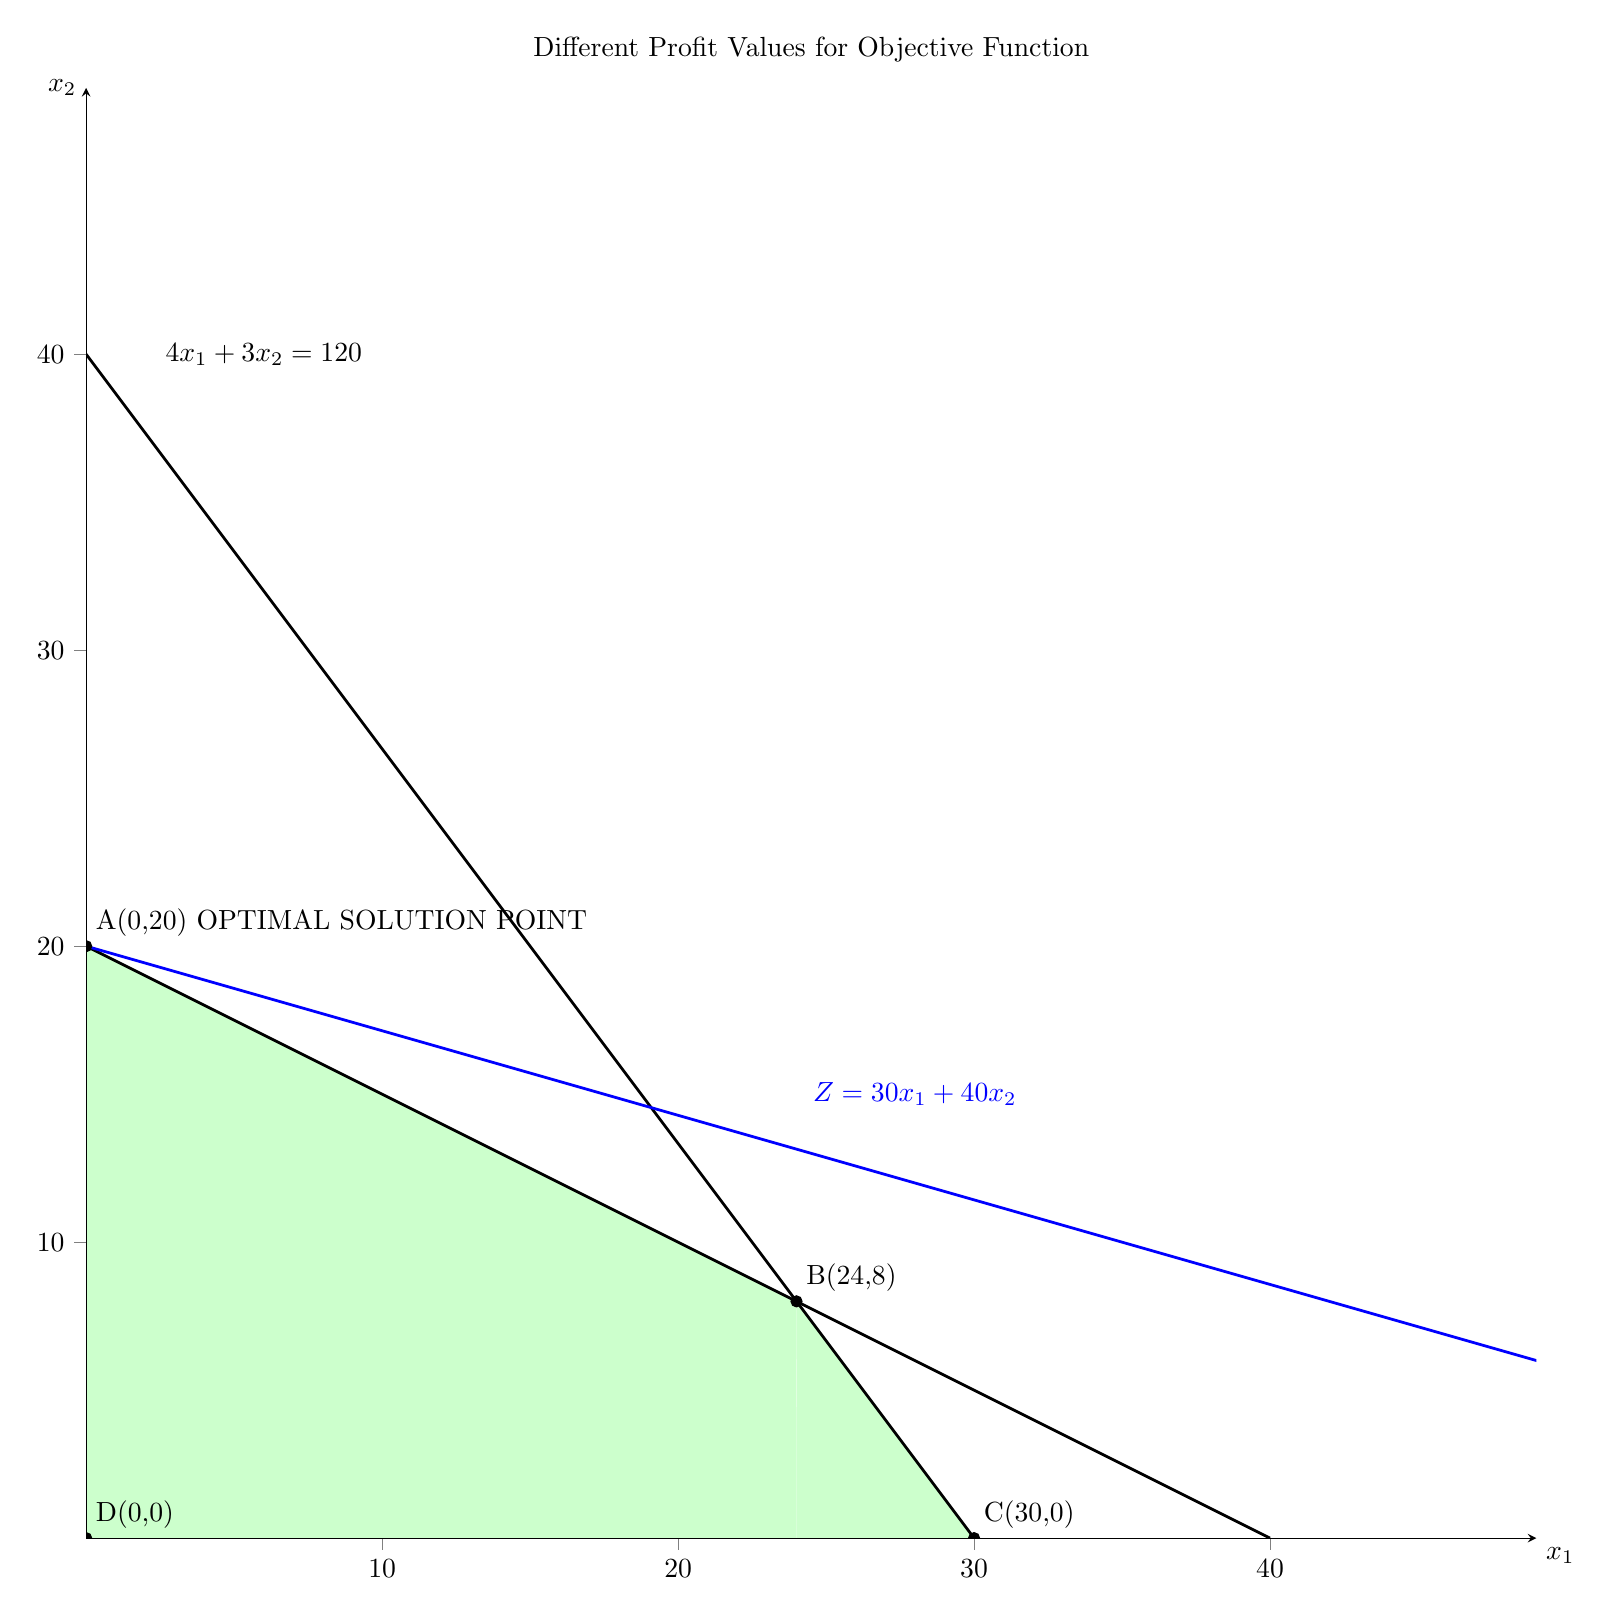
\begin{tikzpicture} [scale=1.0]
  \begin{axis}[
    name = plot1,
    title=Different Profit Values for Objective Function,
    width = 20cm, 
    height = 20cm,
    axis lines=left,
    axis equal image,
    axis on top = true, axis x line = middle, axis y line = middle,
    xmin = 0, ymin = 0, xmax = 49, ymax = 49,
    /pgfplots/xtick = {0,10,...,40},
    /pgfplots/ytick = {0,10,...,40},
    tick align = outside,
    xlabel = {$x_1$}, xlabel style = {at={(ticklabel* cs:1)},anchor = north west},
    ylabel = {$x_2$}, ylabel style = {at={(ticklabel* cs:1)},anchor = east},
    %legend entries={Constraint 1,Constraint 2,Constraint 3},
    ]
    %\addplot+[name path=Constraint1,red, line width = 1] coordinates {(0,50)(50,0)} node {$A$};
    %\addplot+[name path=Constraint1, line width = 1] coordinates {(0,50)(50,0)} node[pin=45:{B}]{};
    \path[name path=Zero]
      (\pgfkeysvalueof{/pgfplots/xmin},0) --
      (\pgfkeysvalueof{/pgfplots/xmax},0);
    \addplot[black,sharp plot, name path=Constraint1, line width = 1] coordinates {(0,20)(40,0)}; % 1
    \addplot[black,sharp plot, name path=Constraint2, line width = 1] coordinates {(0,40)(30,0)}; % 2
%    \node at (44,2) {$x_1 + 2x_2 = 40$};
    \node at (6,40) {$4x_1 + 3x_2 = 120$};
    \node [blue] at (28,15) {$Z = 30x_1 + 40x_2$};

%    \addplot[red!40,dashed, name path=Objective1, line width = 1] coordinates {(0,8)(10,0)};
%    \addplot[red!40,dashed, name path=Objective2, line width = 1] coordinates {(0,16)(20,0)};
%    \addplot[red!40,dashed, name path=Objective3, line width = 1] coordinates {(0,24)(30,0)};
%    \addplot[red!40,dashed, name path=Objective4, line width = 1] coordinates {(0,32)(40,0)};
%    \addplot[red,sharp plot, name path=ObjectiveA, line width = 1] coordinates {(0,27.2)(34,0)}; % Objective function A
%    \addplot[blue,sharp plot, name path=ObjectiveB, line width = 1] coordinates {(0,105)(30,0)}; % Objective function B
    \addplot[blue,sharp plot, name path=ObjectiveC, line width = 1] coordinates {(0,20)(70,0)}; % Objective function C
        
    %\addplot[green!20] fill between[of=Constraint1 and Zero,soft clip={domain=0:40}];
    %\addplot[fill opacity=0.50,blue!40] fill between[of=Constraint2 and Zero];

    \filldraw[black] (0,20) circle (2pt) node[anchor=south west] {A(0,20) OPTIMAL SOLUTION POINT};
    \filldraw[black] (24,8) circle (2pt) node[anchor=south west] {B(24,8)};
    \filldraw[black] (30,0) circle (2pt) node[anchor=south west] {C(30,0)};
    \filldraw[black] (0,0) circle (2pt) node[anchor=south west] {D(0,0)};
    \addplot[green!20] fill between[of=Constraint1 and Zero,soft clip={domain=0:24}];
    \addplot[green!20] fill between[of=Constraint2 and Zero,soft clip={domain=24:30}];

    %\node at (30,30) {Point A, $x_1 = 0, x_2 = 20, Z = 1000$};
    %\node at (30,28) {Point B, $x_1 = 24, x_2 = 8, Z = 1360$};
    %\node at (30,26) {Point C, $x_1 = 30, x_2 = 0, Z = 1200$};
    %\node at (30,24) {Point D, $x_1 = 0, x_2 = 0, Z = 0$};    

    %\draw[->] (24,12) -- (24,10);
    %\node at (26,13) {OPTIMAL POINT};
  \end{axis}
\end{tikzpicture}

% ------------------------------------------------------------------------------------------------------------------------

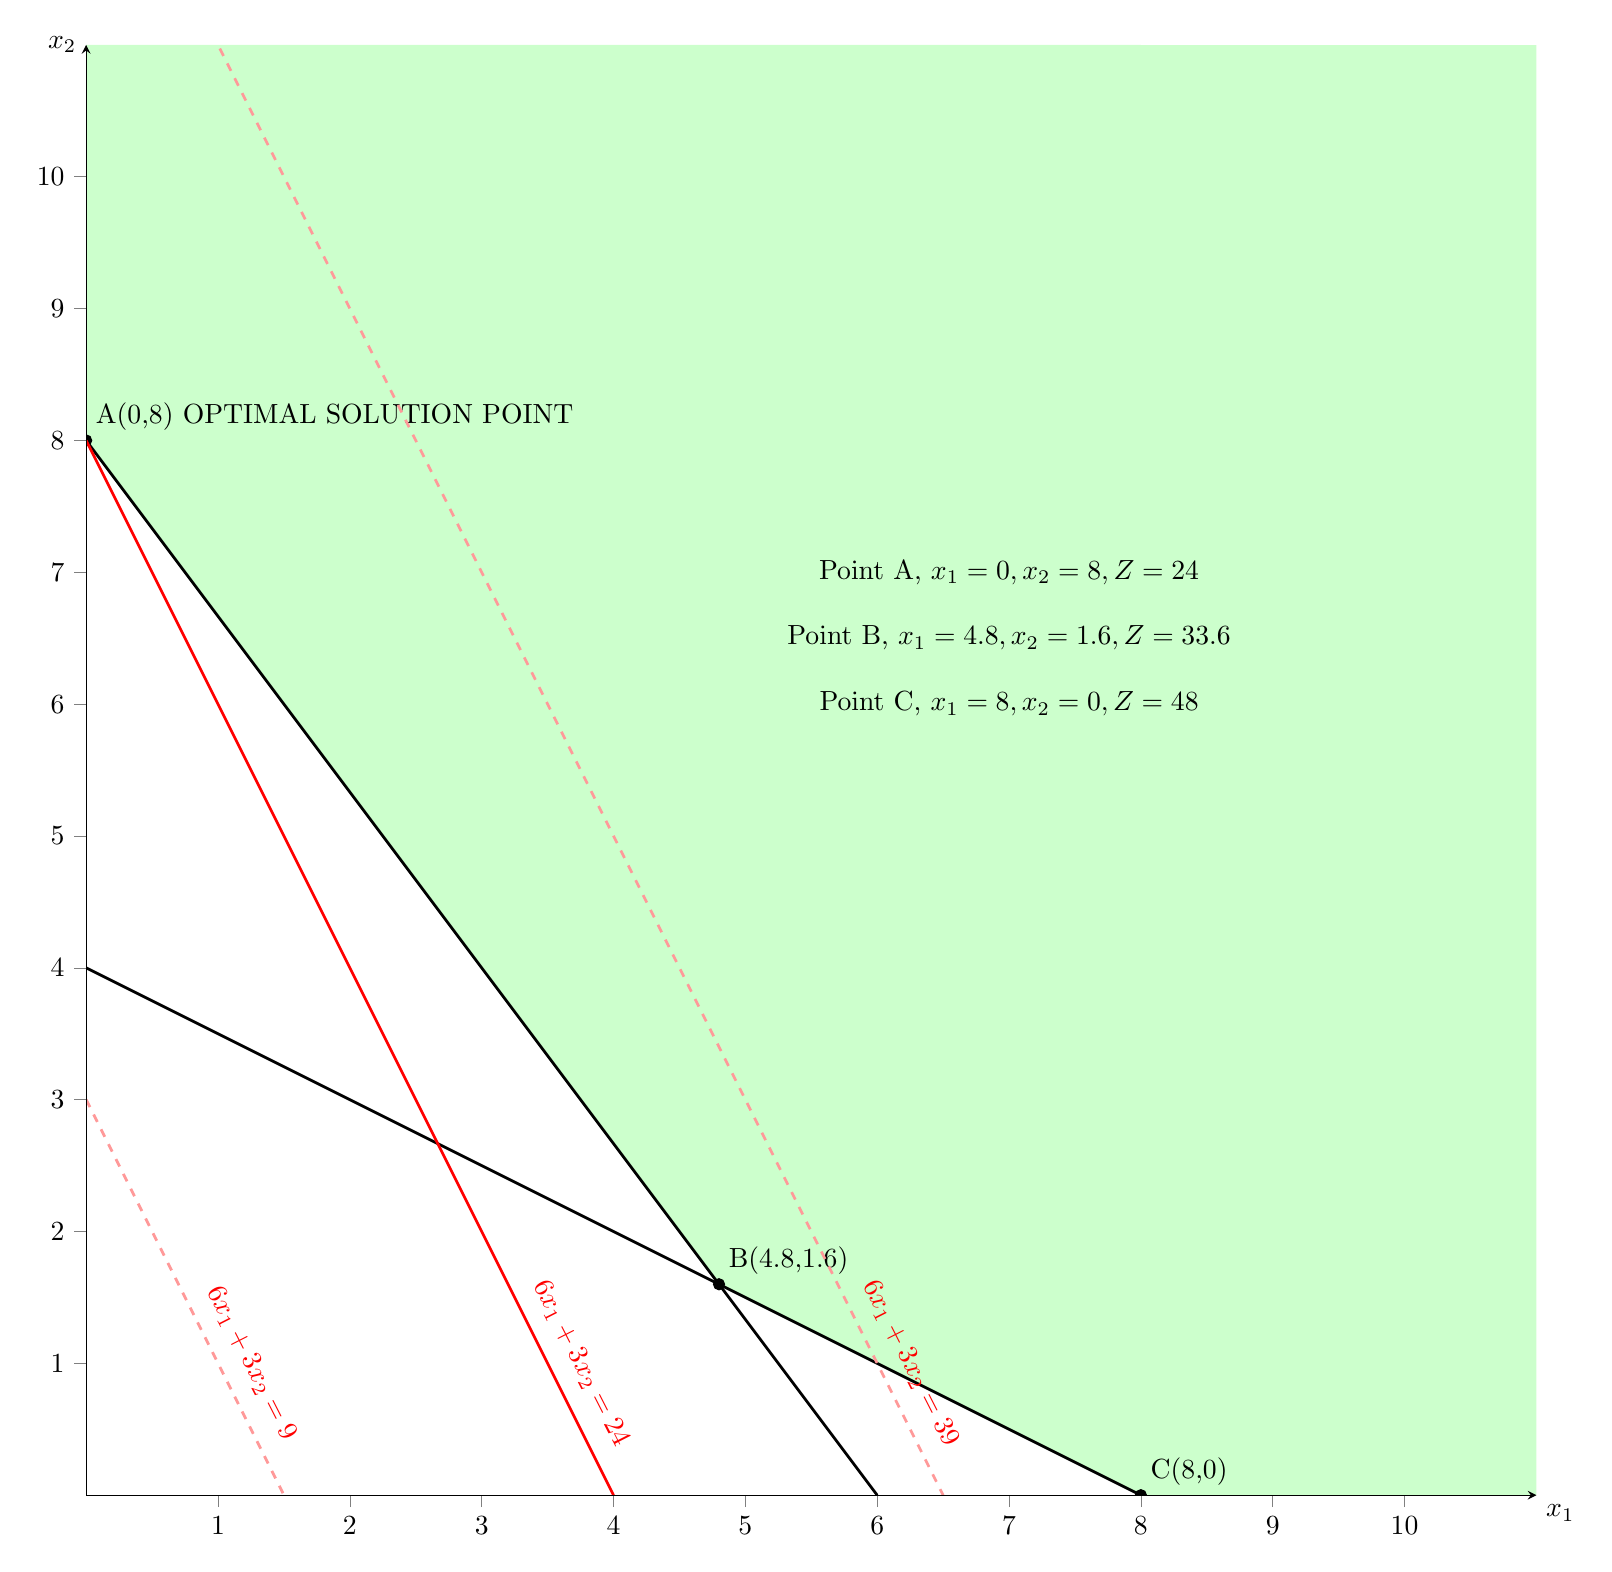
\begin{tikzpicture} [scale=1.0]
  \begin{axis}[
    name = plot2,
%    title=Maximization problem,
    width = 20cm, 
    height = 20cm,
    axis lines=left,
    axis equal image,
    axis on top = true, axis x line = middle, axis y line = middle,
    xmin = 0, ymin = 0, xmax = 11, ymax = 11,
    /pgfplots/xtick = {0,1,...,10},
    /pgfplots/ytick = {0,1,...,10},
    tick align = outside,
    xlabel = {$x_1$}, xlabel style = {at={(ticklabel* cs:1)},anchor = north west},
    ylabel = {$x_2$}, ylabel style = {at={(ticklabel* cs:1)},anchor = east},
    %legend entries={Constraint 1,Constraint 2,Constraint 3},
    ]
    %\addplot+[name path=Constraint1,red, line width = 1] coordinates {(0,50)(50,0)} node {$A$};
    %\addplot+[name path=Constraint1, line width = 1] coordinates {(0,50)(50,0)} node[pin=45:{B}]{};
    \path[name path=Zero]
      (\pgfkeysvalueof{/pgfplots/xmin},0) --
      (\pgfkeysvalueof{/pgfplots/xmax},0);
    \path[name path=Top]
      (\pgfkeysvalueof{/pgfplots/xmin},11) --
      (\pgfkeysvalueof{/pgfplots/xmax},11);
      
    \addplot[black,sharp plot, name path=Constraint1, line width = 1] coordinates {(0,8)(6,0)}; % 1
    \addplot[black,sharp plot, name path=Constraint2, line width = 1] coordinates {(0,4)(8,0)}; % 2
    \node at (6,40) {$4x_1 + 3x_2 = 120$};
    \node at (44,2) {$x_1 + 2x_2 = 40$};

    %\addplot[red!40,dashed, name path=Objective1, line width = 1] coordinates {(0,8)(10,0)};
    %\addplot[red!40,dashed, name path=Objective2, line width = 1] coordinates {(0,16)(20,0)};
    %\addplot[red!40,dashed, name path=Objective3, line width = 1] coordinates {(0,24)(30,0)};
    %\addplot[red!40,dashed, name path=Objective4, line width = 1] coordinates {(0,32)(40,0)};
%    \addplot[red,sharp plot, name path=ObjectiveA, line width = 1] coordinates {(0,8)(4,0)}; % Objective function A
    %\addplot[blue,sharp plot, name path=ObjectiveB, line width = 1] coordinates {(0,105)(30,0)}; % Objective function B
    %\addplot[green,sharp plot, name path=ObjectiveC, line width = 1] coordinates {(0,20)(70,0)}; % Objective function C
        
    %\addplot[green!20] fill between[of=Constraint1 and Zero,soft clip={domain=0:40}];
    %\addplot[fill opacity=0.50,blue!40] fill between[of=Constraint2 and Zero];

    \filldraw[black] (0,8) circle (2pt) node[anchor=south west] {A(0,8) OPTIMAL SOLUTION POINT};
    \filldraw[black] (4.8,1.6) circle (2pt) node[anchor=south west] {B(4.8,1.6)};
    \filldraw[black] (8,0) circle (2pt) node[anchor=south west] {C(8,0)};
    %\filldraw[black] (0,0) circle (2pt) node[anchor=south west] {D(0,0)};
    
    \addplot[green!20] fill between[of=Constraint1 and Top,soft clip={domain=0:4.8}];
    \addplot[green!20] fill between[of=Constraint2 and Top,soft clip={domain=4.8:8}];
    \addplot[green!20] fill between[of=Zero and Top,soft clip={domain=8:11}];

    \addplot[red!40,dashed, name path=Objective2, line width = 1] coordinates {(0,3)(1.5,0)};
   	\node [rotate=-63,red] at (1.25,1) {$6x_1 + 3x_2 = 9$};

    \addplot[red!40,dashed, name path=Objective2, line width = 1] coordinates {(0,13)(6.5,0)};
   	\node [rotate=-63,red] at (6.25,1) {$6x_1 + 3x_2 = 39$};

    \addplot[red,sharp plot, name path=ObjectiveA, line width = 1] coordinates {(0,8)(4,0)}; % Objective function A
   	\node [rotate=-63,red] at (3.75,1) {$6x_1 + 3x_2 = 24$};

    \node at (7,7) {Point A, $x_1 = 0, x_2 = 8, Z = 24$};
    \node at (7,6.5) {Point B, $x_1 = 4.8, x_2 = 1.6, Z = 33.6$};
    \node at (7,6) {Point C, $x_1 = 8, x_2 = 0, Z = 48$};
    %\node at (30,24) {Point D, $x_1 = 0, x_2 = 0, Z = 0$};    

    %\draw[->] (24,12) -- (24,10);
    %\node at (26,13) {OPTIMAL POINT};
  \end{axis}
\end{tikzpicture}





















\end{document}